\documentclass[10pt, a4paper, italian]{article}
\usepackage[T1]{fontenc}
\usepackage[utf8]{inputenc}
\usepackage{amsmath, amssymb, amsthm, thmtools, amsfonts, mathtools}
\usepackage{nicefrac}
\usepackage{calc}
\usepackage[pdftex, hyperindex, plainpages=false]{hyperref}
\usepackage[nameinlink]{cleveref} %load before classicthesis (clash)
%\usepackage[nochapters,pdfspacing]{classicthesis}
\usepackage{siunitx}
\usepackage[siunitx]{circuitikz}

\usepackage[a4paper]{geometry}
\usepackage{float}
\usepackage{mdframed}
\usepackage{titling}
\usepackage{booktabs}
\usepackage{graphicx}
\usepackage{caption, subcaption}
\usepackage{xcolor}
\usepackage[italian]{babel}
\usepackage{pgfplots}
\usepackage{listings}
%\usepackage{lmodern}
\usepackage{url}
\usepackage{enumitem}
\usepackage{tikz} %loads after classicthesis (xcolor incompat)

% lets graphicx know path where figures to be included are found
\graphicspath{{../figs/}}
\makeatletter
\def\input@path{{../figs/}}
%or: \def\input@path{{/path/to/folder/}{/path/to/other/folder/}}
\makeatother

% tikz pgf plots setup
\usepgfplotslibrary{external}
\pgfplotsset{compat=1.15}
%\tikzexternalize

% spaces and significant digits/figures for measurements
\sisetup{free-standing-units, space-before-unit, number-unit-product = \;,
scientific-notation = false, round-mode = figures, round-precision = 1,}

% turns all (hyperlinked) references black [default is blue]
\hypersetup{
	linktoc=all,
	colorlinks=true,
	linkcolor=black
}

% code listings config
%\lstset{
%language=Python,
%basicstyle=\ttfamily,
%columns=fullflexible,
%keepspaces=true,
%}

% mdframed (for boxed text) configuration
\mdfsetup{linewidth=0.6pt}

% Default fixed font does not support bold face
\DeclareFixedFont{\ttb}{T1}{txtt}{bx}{n}{12} % for bold
\DeclareFixedFont{\ttm}{T1}{txtt}{m}{n}{12}  % for normal

% Custom colors
\usepackage{color}
\definecolor{deepblue}{rgb}{0,0,0.5}
\definecolor{deepred}{rgb}{0.6,0,0}
\definecolor{deepgreen}{rgb}{0,0.5,0}

% Commands 
\newcommand{\executeiffilenewer}[3]{%
	\ifnum\pdfstrcmp{\pdffilemoddate{#1}}%
		{\pdffilemoddate{#2}}>0%
	{\immediate\write18{#3}}\fi%
}
% input .svg --> .pdf_tex graphs
%\newcommand{\includesvg}[1]{%
%	\executeiffilenewer{#1.svg}{#1.pdf}%
%	{inkscape -z -D --file=#1.svg %
%	--export-pdf=#1.pdf --export-latex}%
%	\input{#1.pdf_tex}%
%}
% Thanks UniPi's Department of Physics E. Fermi
\newcommand{\thanksdf}{(\thanks{Dipartimento di Fisica E.~Fermi,%
Universit\`a di Pisa - Pisa, Italy.}\;)}

% hyperlink to email address
\newcommand{\mail}[1]{\href{mailto:#1}{\textsf{#1}}}

% \vec for bold vectors, instead of overarrows (now "\arrvec")
\let\arrvec=\vec
\renewcommand{\vec}[1]{\boldsymbol #1}
% replaces straight phi with slanted phi
\renewcommand{\phi}{\varphi}
% replaces straight eps with curved epsilon
\newcommand{\eps}{\varepsilon}
% abbreviation for (sub_/super^)scripts of \lim, \sum,... in inline math
\newcommand{\ds}{\displaystyle}

% blackboard/number set letters
\newcommand{\CC}{\mathbb C}
\newcommand{\HH}{\mathbb H}
\newcommand{\KK}{\mathbb K}
\newcommand{\NN}{\mathbb N}
\newcommand{\PP}{\mathbb P}
\newcommand{\QQ}{\mathbb Q}
\newcommand{\RR}{\mathbb R}
\newcommand{\ZZ}{\mathbb Z}

\newcommand{\Abs}[1]{{\left\Vert #1\right\Vert}}
\newcommand{\enclose}[1]{{\left( #1 \right)}}
\newcommand{\Enclose}[1]{{\left[ #1 \right]}}
\newcommand{\floor}[1]{\left\lfloor #1 \right\rfloor}
\newcommand{\ceil}[1]{\left\lceil #1 \right\rceil}
\newcommand{\To}{\rightrightarrows}

% Math operators
\DeclareMathOperator{\divergence}{div}
\renewcommand{\div}{\divergence}
\DeclareMathOperator{\Imaginarypart}{Im}
\renewcommand{\Im}{\Imaginarypart}
\DeclareMathOperator{\Realpart}{Re}
\renewcommand{\Re}{\Realpart}
%\DeclareMathOperator{\arg}{arg}
\DeclareMathOperator{\tg}{tg}
\DeclareMathOperator{\arctg}{arctg}
\DeclareMathOperator{\settsinh}{settsinh}
\DeclareMathOperator{\settcosh}{settcosh}
\DeclareMathOperator{\tr}{tr}
\DeclareMathOperator{\im}{im}
\DeclareMathOperator{\sgn}{sgn}
\DeclareMathOperator{\diag}{diag}

\DeclarePairedDelimiter{\norm}{\lVert}{\rVert}
\DeclarePairedDelimiter{\scalar}{\langle}{\rangle}

% Logarithm with arbitrary base.
% -> log_10
\newcommand{\llog}[1][10]{\log_{#1}}

% Absolute value.
% -> |x|
\newcommand{\abs}[1]{\left| #1 \right|}

% Powers.
% -> x^a
\newcommand{\power}[2][2]{\left( #2 \right)^{#1}}

% Square.
% -> x^2
\newcommand{\sq}[1]{\power[2]{#1}}

% Expansion of the binomial coefficient.
% -> n1!/(n2!(n1 - n2)!)
\newcommand{\binomexpr}[2]{\frac{#1!}{#2!(#1 - #2)!}}

% Expression evaluation at a given point with square brackets.
% -> [x]_{a}
\newcommand{\at}[2]{\left[ #1\right]_{\makebox[-1pt][l]{${\scriptstyle#2}$}}}

% Expression evaluation in an interval.
% -> [x] _{a}^{b}
\newcommand{\eval}[3]{\left.#1%
  \right|_{\makebox[-1pt][l]{${\scriptstyle#2}$}}^{\makebox[-1pt][l]{${\scriptstyle#3}$}}}

% Upright d in math mode (for differentials).
% -> d
\newcommand{\ud}{\mathrm{d}}

% Differential.
% -> dx
\newcommand{\diff}[1][x]{\,\ud{#1}}

% Base command for defining derivatives.
% -> df/dx or d^kf/dx^k
\newcommand{\basederivative}[4][]{%
  \displaystyle%
  \ifx\\#1\\\frac{#4#2}{#4#3}%
  \else%
  \frac{#4^#1#2}{#4#3^#1}%
  \fi%
}

% Total derivative.
% -> df/dx(x) or d^kf/dx^k(x)
\newcommand{\td}[4][]{%
  \basederivative[#1]{#2}{#3}{\ud}%
  \ifx\\#4\\%
  \else%
  \mkern-4mu\left(#4\right)%
  \fi%
}

% Partial derivative.
% -> df/dx(x) or d^kf/dx^k(x)
\newcommand{\pd}[4][]{%
  \basederivative[#1]{#2}{#3}{\partial}%
  \ifx\\#4\\%
  \else%
  \mkern-4mu\left(#4\right)%
  \fi%
}

\newcommand{\intinf}{\int_{-\infty}^{\infty}\!\!\!}

\newcommand{\cinterval}[2]{\left[\, #1,~#2 \,\right]}

\newcommand{\linterval}[2]{\left[\, #1,~#2 \,\right)}

\newcommand{\rinterval}[2]{\left(\, #1,~#2 \,\right]}

\newcommand{\ointerval}[2]{\left(\, #1,~#2 \,\right)}

\newcommand{\prob}[1]{\displaystyle P\left(#1\right)}

\newcommand{\pvalue}{\emph{$p$-value}}

\newcommand{\cond}{\,|\,}

\newcommand{\expect}[1]{\displaystyle E\left[#1\right]}

\newcommand{\mom}[2][]{\displaystyle {\cal M}_{#2}\ifx\\#1\\\else(#1)\fi}

\newcommand{\momalg}[1]{\displaystyle \lambda_{#1}}

\newcommand{\momcen}[1]{\displaystyle \mu_{#1}}

\newcommand{\skewness}{\displaystyle \gamma_1}

\newcommand{\kurtosis}{\displaystyle \gamma_2}

\newcommand{\charf}[1][x]{\phi_{#1}}

\newcommand{\momgenf}[1][x]{M_{#1}}

\newcommand{\fwhm}{{\scriptstyle \textsc{FWHM}}}

\newcommand{\hwhm}{{\scriptstyle \textsc{HWHM}}}

\newcommand{\median}{\mu_{\nicefrac{1}{2}}}

\newcommand{\var}[1]{\ensuremath{\text{Var}\left(#1\right)}}

\newcommand{\cov}[2]{\ensuremath{\text{Cov}\left(#1, #2\right)}}

\newcommand{\corr}[2]{\ensuremath{\text{Corr}\left(#1, #2\right)}}

\newcommand{\like}{\mathcal L}

\newcommand{\likelihood}[2][]{\like\ifx\\#2\\\else(#2\ifx\\#1\\\else;#1\fi)\fi}

\newcommand{\chisq}{\ensuremath{\chi^2}}

\newcommand{\chisquare}[2][]{\chisq\ifx\\#2\\\else(#2\ifx\\#1\\\else;#1\fi)\fi}

\newcommand{\loglikelihood}[2][]{\log\likelihood[#1]{#2}}

\newcommand{\pdf}[3][]{#2(#3\ifx\\#1\\\else;#1\fi)}

\newcommand{\binomialpdf}[2][]{\pdf[#1]{\mathcal B}{#2}}

\newcommand{\multinomialpdf}[2][]{\pdf[#1]{\mathcal M}{#2}}

\newcommand{\poissonpdf}[2][]{\pdf[#1]{\mathcal P}{#2}}

\newcommand{\uniformpdf}[2][]{\pdf[#1]{u}{#2}}

\newcommand{\exponentialpdf}[2][]{\pdf[#1]{\varepsilon}{#2}}

\newcommand{\gausspdf}[2][]{\pdf[#1]{N}{#2}}

\newcommand{\chisquarepdf}[2][]{\pdf[#1]{\wp}{#2}}

\newcommand{\cauchypdf}[2][]{\pdf[#1]{c}{#2}}

\newcommand{\erf}[1]{\ensuremath{\text{erf}\left(#1\right)}}

\newcommand{\dccases}[4][]{#2 \ifx\\#2\\\else=\fi %
  \begin{cases}
    \displaystyle #3 & \text{per variabili discrete}\\
    \displaystyle #4 & \text{per variabili continue}#1
  \end{cases}
}
% sub/super-scriptable for all symbol as math operator 
\newcommand\Scaleforall[1]{\vcenter{\hbox{\scalefont{#1}$\forall$}}}

\DeclareMathOperator*\forevery{%
  \vphantom\sum
  \mathchoice{\Scaleforall{2}}{\Scaleforall{1.4}}{\Scaleforall{1}}{\Scaleforall{0.75}}}
\usepackage{multicol}
\usepackage{diagbox}
\geometry{left=2cm, right=2cm, top=2cm, bottom=2cm}

% indexes subsections with letters, sections with numbers (1.a, 1.b, ...)
\renewcommand{\thesubsection}{\thesection.\alph{subsection}}

% lets graphicx know path where figures to be included are found
\graphicspath{{../figs/}}

\author{Gruppo 1.AC \\ Matteo Rossi, Bernardo Tomelleri}
\title{EsD1: Caratterizzazione di porte logiche e semplici circuiti logici.}
\begin{document}
\date{\today}
\maketitle

\section*{Misura componenti dei circuiti}
\begin{table}[htbp]
\centering
\begin{tabular}{ccc}
\toprule
Resistenze $[\si{\ohm}]$ & $R$ & $\sigma R$ \\
\midrule
\midrule
$R\ped{pot1}$	& 9.53 k	& 0.08 k 		\\
$R\ped{pot2}$	& 9.78 k	& 0.08 k 		\\

\bottomrule     
\end{tabular}
\caption{Valori di resistenza misurati per i componenti passivi dei circuiti
studiati. \label{tab: rmesM}}
\end{table}

Riportiamo per completezza anche il valore della tensione continua di
alimentazione per i circuiti integrati misurata con il multimetro
\begin{align*}
V_{CC} &= 4.99 \pm 0.03 \si{\V} \\
\end{align*}

\subsection*{Nota sul metodo di fit}
Per determinare i parametri ottimali e le rispettive covarianze si \`e
implementato in \verb+Python+ un algoritmo di fit basato sui minimi quadrati
mediante la funzione \emph{curve\_fit} della libreria \texttt{SciPy}.

\setcounter{section}{0}
%=======================
\section*{Parte A: Caratteristiche fisiche delle porte logiche}
Si studia il comportamento delle porte NOT TTL contenute nel circuito
integrato SN7404 misurando le tensioni e correnti di operazione e verificando
che queste rientrino nelle specifiche tecniche riportate nel Data-Sheet del
chip in \cref{fig: SN7404}.
\begin{figure}[htbp]
\centering
    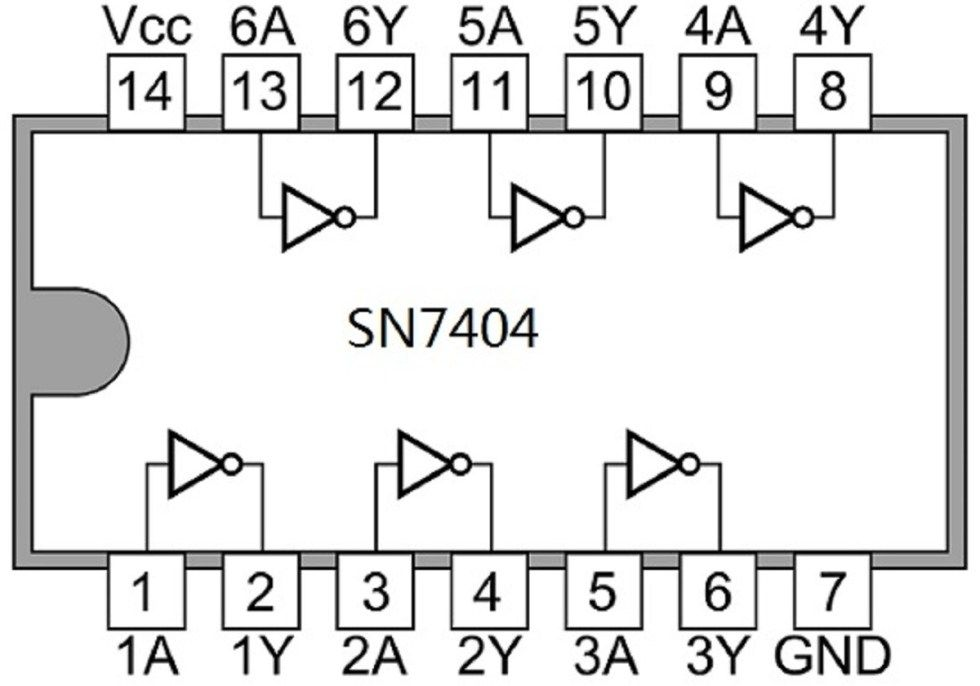
\includegraphics[width=0.3\textwidth]{SN7404}
    \caption{Schema e pedinatura del chip integrato
    quad-NOT SN7404 \label{fig: SN7404}}
\end{figure}

\section{Tensioni di operazione}\label{sec: tens}
Per prima cosa misuriamo i valori delle tensioni di soglia in ingresso e in
uscita (e verifichiamo che rispettino le specifiche di buon funzionamento del
DS) da cui è possibile ottenere una misura del Noise Margin delle porte.

Dalle specifiche del DS si ha che i valori attesi sono: (riportati in
\cref{tab: notDS})
\begin{table}[htbp]
\centering
\begin{tabular}{cccc|c}
\toprule
Parameter  & min & typ & max & [Unit] \\
\midrule
\midrule
$V_{CC}$ &  &  & $7$ & V \\
$V_I$	 &  &  & $5.5$ & V\\
$V_{OH}$ & $2.4$  & $3.4$ & & V \\
$V_{OL}$ &   & $0.2$ & $0.4$ & V \\
$V_{IH}$ & $2$  &  & & V  \\
$V_{IL}$ &  &  & $0.8$ & V \\
$I_{IH}$ &  &  & $40$ & $\si{\micro\A}$ \\
$I_{OH}$ &  &  & $-0.4$ & mA \\
\bottomrule 
\end{tabular}
\caption{Valori delle tensioni e correnti di operazione indicati sul
datasheet dell'integrato SN7404.}
\label{tab: notDS}
\end{table}

in cui $V_O$ e $V_I$ sono definite come le tensioni in uscita e in ingresso
dalla porta logica (le altre diciture indicano se la grandezza a cui facciamo
riferimento corrisponde a uno stato logico alto (H) o basso (L) e quali sono
i massimi o minimi valori garantiti dal costruttore).

\subsection{Misura delle tensioni di soglia dal grafico
$V\ped{out}(V\ped{in})$}
Generiamo una rampa di tensione compresa tra 0-5 V e la inviamo
all'ingresso di una porta NOT per osservare i segnali generati in uscita,
così da ottenere un grafico di $V\ped{out}$ in funzione di $V\ped{in}$.

Abbiamo quindi utilizzato i cursori per misurare $V_{OH}$ e $V_{OL}$, cioè
la tensione che raggiunge l'uscita in saturazione per valore logico H e L
rispettivamente, mentre per misurare $V_{IL}$ e $V_{IH}$ abbiamo misurato le
tensioni in ingresso per cui inizia e finisce la commutazione dell'uscita
secondo lo schema in \cref{fig: trans}:
\begin{figure}[htbp]
\centering
	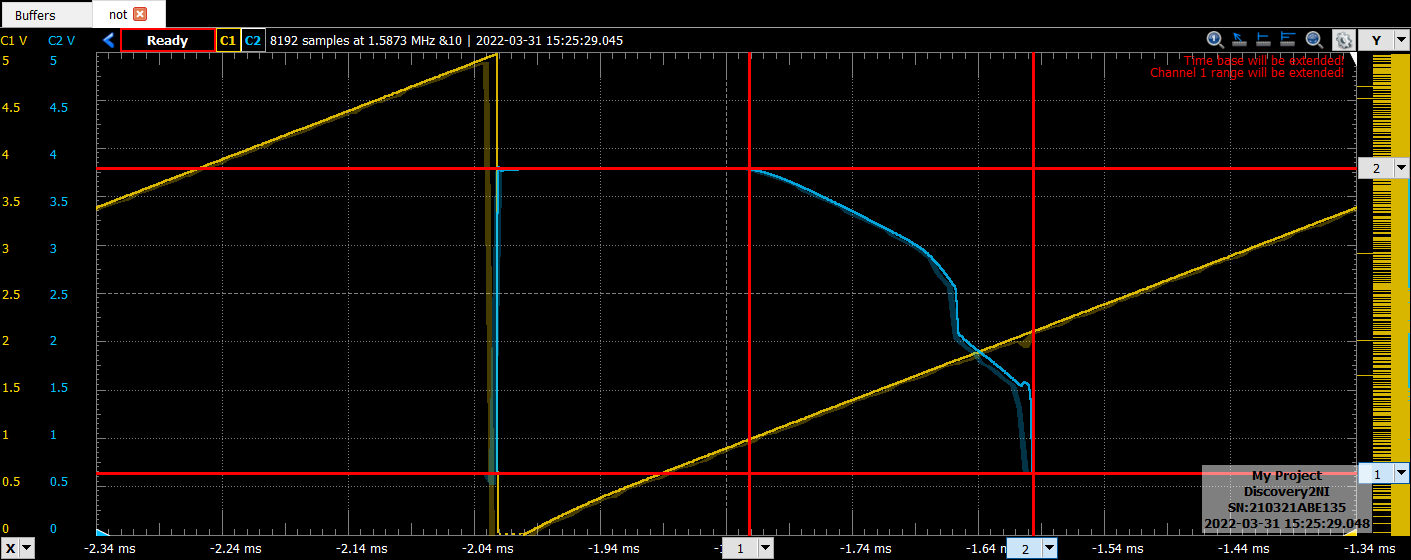
\includegraphics[width=\textwidth]{trans}
	\caption{Schema di come sono stati utilizzati i cursori per misurare le tensioni $V_{OH}$, $V_{OL}$ (cursori orizzontali) e $V_{IH}$, $V_{IL}$ (aiutandosi con i cursori verticali a individuare la fase di transizione H->L)}
	\label{fig: trans}
\end{figure}
\begin{multicols}{2}
    \centering
    $V_{OH} = 3.78 \pm 0.03\; \si{\V}$ \\
	$V_{OL} = 632 \pm 4 \; \si{m\V}$ \\
	$V_{IH} = 2.10 \pm 0.02 \; \si{\V} $\\
	$V_{IL} = 979 \pm 9\; \si{m\V} $\\
    
    $V_{OH} = 3.76 \pm 0.03\; \si{\V}$ \\
	$V_{OL} = 341 \pm 3 \; \si{m\V}$ \\
	$V_{IH} = 1.81 \pm 0.02 \; \si{\V} $\\
	$V_{IL} = 772 \pm 8\; \si{m\V} $\\
\end{multicols}

\begin{figure}[htbp]
\centering
	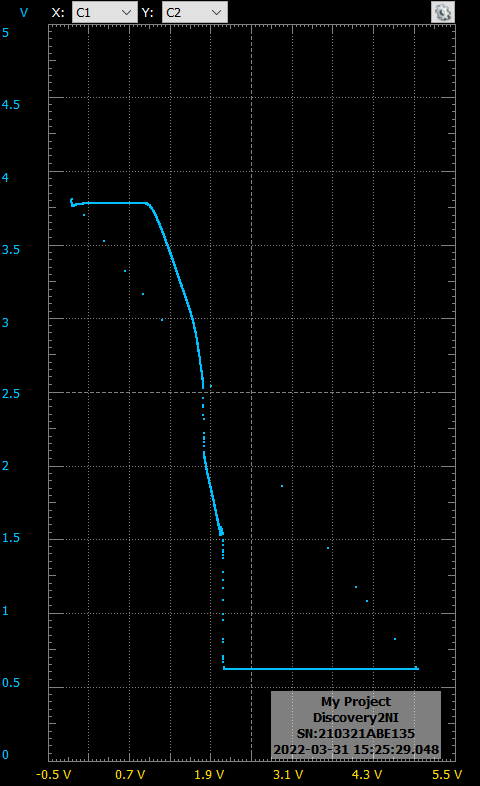
\includegraphics[scale=0.4]{not_xy1}
	\caption{Grafico XY di $V\ped{out}$ in funzione di $V\ped{in}$}
\end{figure}
\begin{figure}[htbp]
\centering
	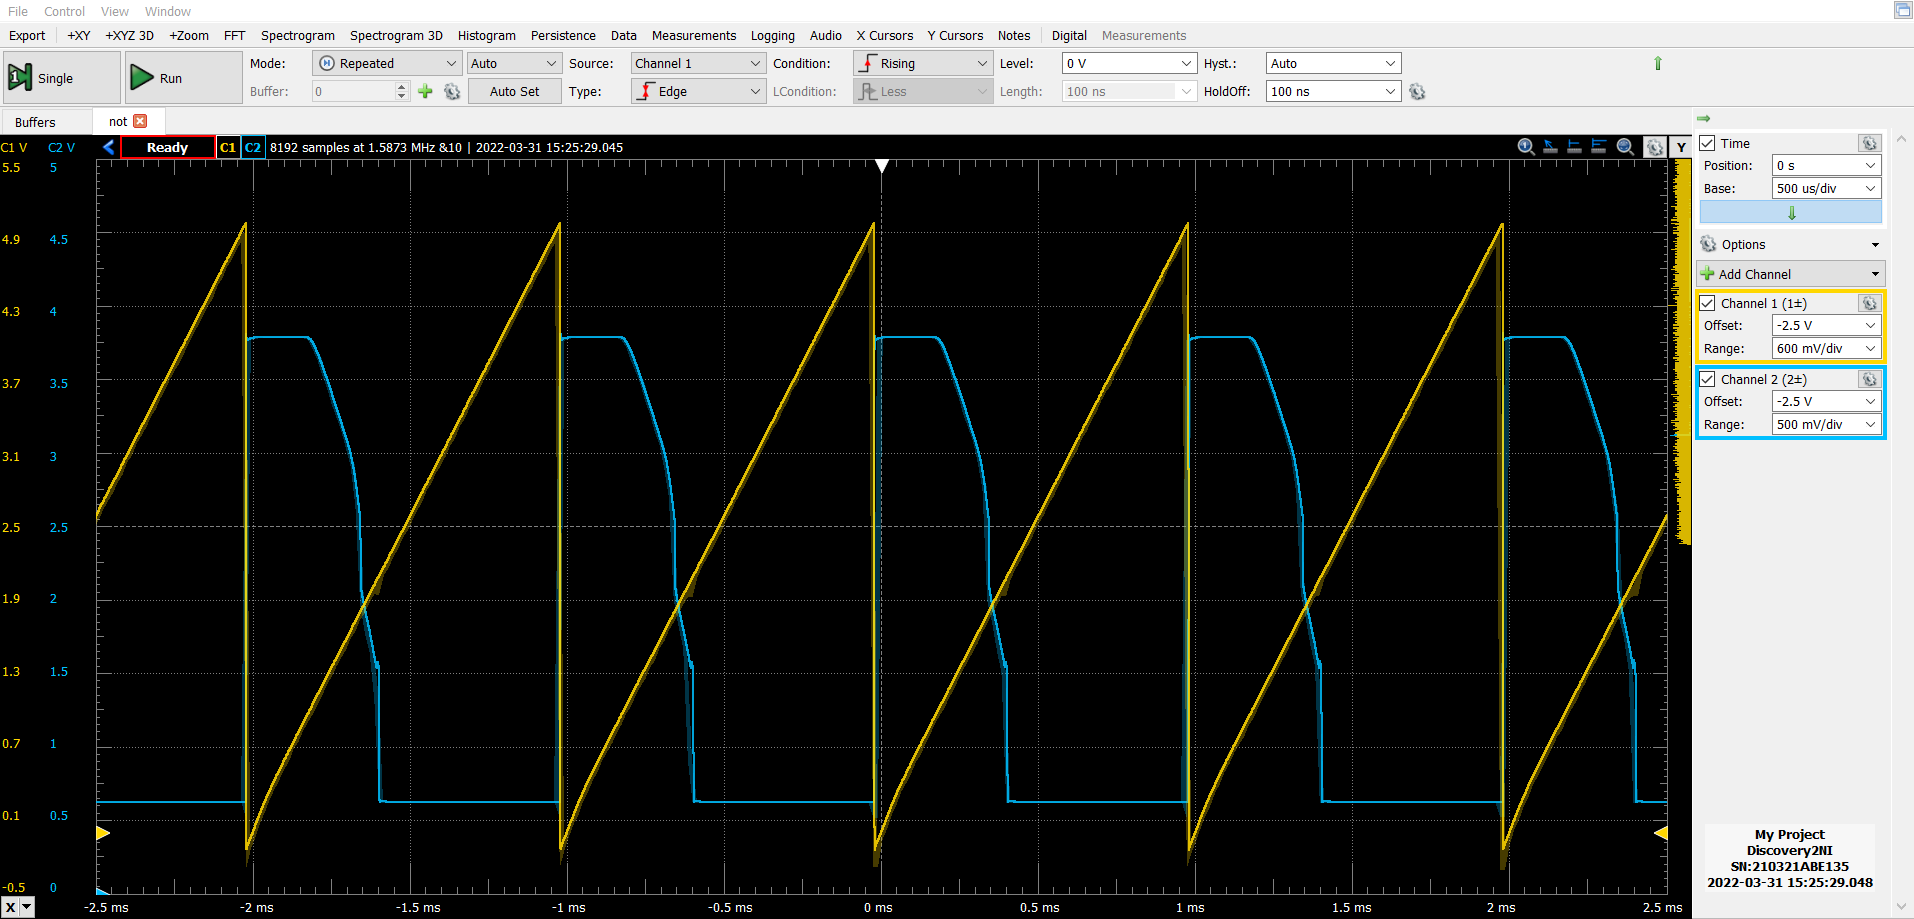
\includegraphics[width=\textwidth]{not_time1}
	\caption{Acquisizione all'oscilloscopio dell'andamento nel tempo dei
	segnali $V\ped{in}$ (CH1, una rampa da 0 a 5 V di frequenza $f = 1$ kHz)
	e $V\ped{out}$ (CH2)}
\end{figure}

Sempre con i cursori abbiamo misurato $V\ped{OH, min}$ dato che il valore
minimo per lo stato alto dell'uscita risultava più basso di
quanto misurato prima; di conseguenza abbiamo spostato il cursore nel punto
in cui la tensione in uscita cambia in maniera più repentina:
\begin{figure}
\centering
	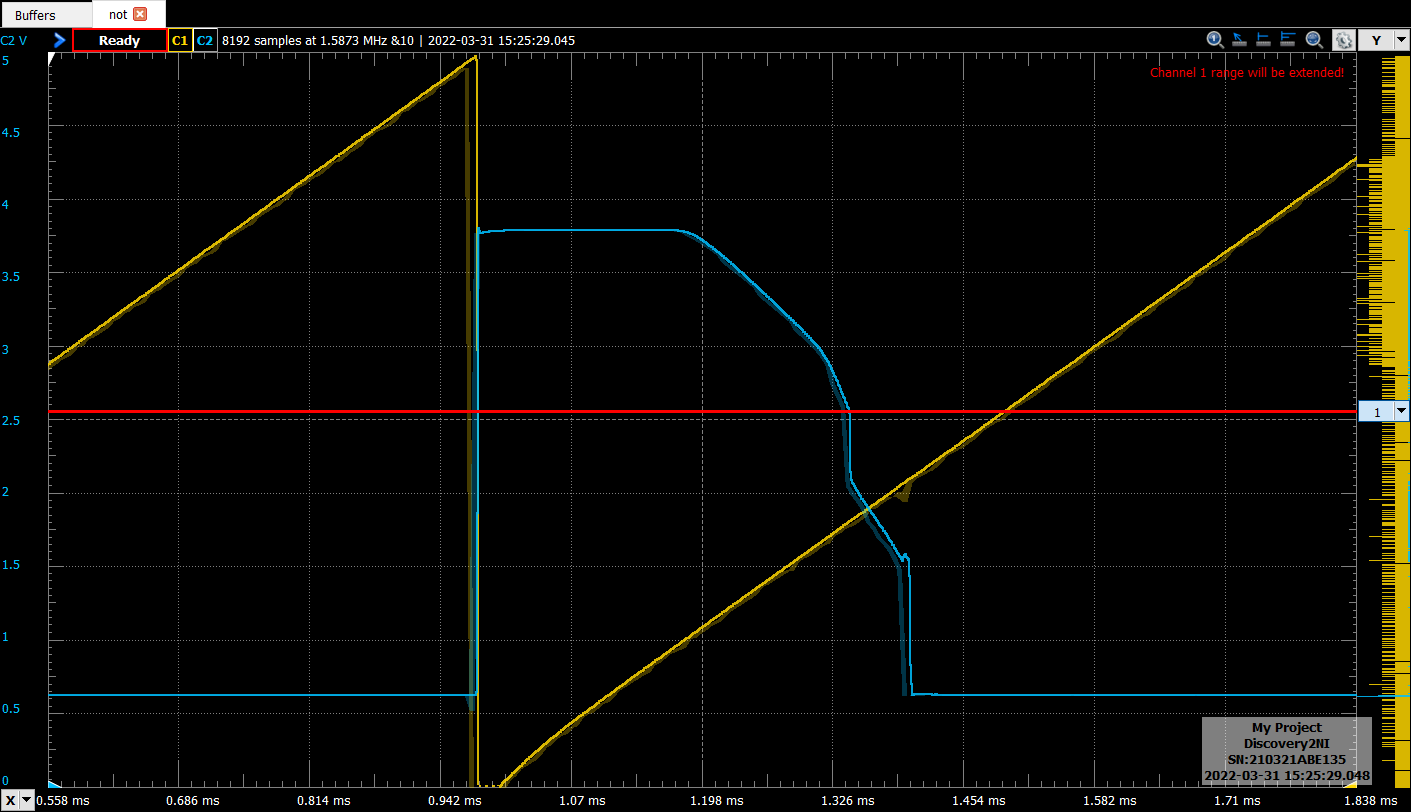
\includegraphics[scale=0.4]{trans1}
	\caption{Schema di come è stata presa la misura di $V\ped{OH, min}$ tramite
	l'utilizzo dei cursori. Si è scelto come valore minimo la tensione
	dell'uscita subito prima del punto di discesa più ripida.}
	\label{fig: trans1}
\end{figure}

Successivamente si sono utilizzati i valori misurati già elencati prima per
ottenere le nostre stime delle tensioni di soglia.
Per il primo integrato:
\begin{multicols}{2}
    \centering
    $V\ped{OH, min}=$ 2.53 $\pm$ 0.03 V\\
    $V\ped{IH, min}=$ 2.10 $\pm$ 0.02 V\\
    
    $V\ped{IL, max}=$ 979 $\pm$ 9 mV\\
    $V\ped{OL, max}=$ 632 $\pm$ 4 mV\\
\end{multicols}
mentre per il secondo:
\begin{multicols}{2}
    \centering
    $V\ped{OH, min}=$ 2.40 $\pm$ 0.03 V\\
    $V\ped{IH, min}=$ 1.81 $\pm$ 0.02 V\\
%    $NM_H=$ 0.60 $\pm$ 0.04 V
    
    $V\ped{IL, max}=$ 772 $\pm$ 8 mV\\
    $V\ped{OL, max}=$ 341 $\pm$ 3 mV\\
%    $NM_L=$ 0.43 $\pm$0.01 V
\end{multicols}

Da cui troviamo le nostre stime dei valori delle soglie di rumore (Noise
Margin High e Low) per le porte NOT studiate, definite come
\begin{multicols}{2}
\begin{align*}
NM_H = V\ped{OH, min} - V\ped{IH, min} &= (0.43 \pm 0.04) \; \si{\V} \\
    &= (0.60 \pm 0.03) \; \si{\V}
\end{align*}

\begin{align*}    
NM_L = V\ped{IL, max} - V\ped{OL, max} &= (0.35 \pm 0.02) \; \si{\V} \\
    &= (0.43 \pm 0.02) \; \si{\V}
\end{align*}
\end{multicols}

\subsection{Valori attesi per le soglie di rumore}
Estrapolando i corrispettivi valori dal datasheet, e assumendo che ogni porta
logica abbia i medesimi parametri delle altre presenti nello stesso integrato
possiamo allora ricavare i valori attesi dei Noise Margin High e Low:
\begin{align*}
NM_H = 2.4 - 2 = 0.4 \; \si{\V} \\
NM_L = 0.8 - 0.4 = 0.4 \; \si{\V}
\end{align*}

\subsection{Confronto dei risultati}
Le nostre misure risultano compatibili con le aspettative entro gli intervalli
ammessi dal datasheet per il buon funzionamento del componente, dunque anche
le grandezze derivate risultano in accordo con le aspettative.

\section{Misura (statica) del Fan-out}
Chiamiamo Fan-Out il massimo numero di porte che una singola porta è in grado
di pilotare rimanendo entro le specifiche di funzionamento del datasheet, lo
si è definito come
\[
\text{FO}= \abs{\frac{I\ped{IH, max}}{I\ped{OH, max}}}
\]

\subsection{Misura della corrente in ingresso alla porta NOT nello stato alto}
Misuriamo la corrente $I\ped{IH, max}$ per entrambi gli integrati collegando
l'amperometro in serie tra l'ingresso della porta logica e l'uscita del
canale WaveGen1 dell'AD2, quindi generando in questo canale una tensione
continua di livello alto pari a 5 V, da cui si trova
\begin{align*}
    I\ped{IH, 1} &= 16 \pm 1 \; \si{\micro\A} \\
    I\ped{IH, 2} &= 10 \pm 1 \; \si{\micro\A} \\   
\end{align*}
Che risultano essere compatibili entro i limiti del datasheet.

\subsection{Misura della corrente in uscita dalla porta NOT per VOH tipico}
Successivamente abbiamo inviato all'ingresso della porta un segale DC a 0 V
(sempre utilizzando il canale WG1) e abbiamo inserito un potenziometro da
$10 \; \si{k\ohm}$ in serie all'uscita di questa per misurare la corrente che
scorre attraverso questa ``resistenza di carico'' regolabile in modo da
avere quando una tensione in uscita dalla porta corrispondente al valore
tipico di $V_{OH}= 3.40 \pm 0.03 \; \si{\V}$.
\begin{align*}
    I\ped{OH, 1} &= 495 \pm 4 \; \si{\micro\A} \\
    I\ped{OH, 2} &= 315 \pm 3 \; \si{\micro\A} \\   
\end{align*}

\subsection{Misura della corrente in uscita dalla porta NOT per VOH misurato}
Per completezza abbiamo impostato il potenziometro in modo che la tensione
$V_{OH}$ risultasse (entro l'incertezza) pari a $V\ped{OH, min}$ e
$V\ped{OH, sat}$ misurati precedentemente e si è ripetuta la misura di
$I_{OH}$ per entrambi gli integrati:

Riportiamo le nostre misure per $V_{OH,sat}= 3.78 \pm 0.03 \; \si{\V}$
\begin{align*}
    I\ped{OH, 1} &= 453 \pm 4 \; \si{\micro\A} \\
    I\ped{OH, 2} &= 275 \pm 2 \; \si{\micro\A} \\   
\end{align*}

quindi per $V\ped{OH, min}= 2.50 \pm 0.02 \; \si{\V}$
\begin{align*}
    I\ped{OH, 1} &= 782 \pm 6 \; \si{\micro\A} \\
    I\ped{OH, 2} &= 552 \pm 5 \; \si{\micro\A} \\   
\end{align*}

\subsection{Misura indiretta del fan-out}
Dalle misure di corrente sui due integrati ricaviamo finalmente che:
\begin{align*}
    \text{FO}_1 &= 31 \pm 2 \\
    \text{FO}_2 &= 32 \pm 3 \\
\end{align*}
Mentre usando le correnti misurate per gli altri valori di $V_{OH}$:
\begin{align*}
    \text{FO}\ped{1, sat} &= 28 \pm 2 \\
    \text{FO}\ped{2, sat} &= 28 \pm 3 \\
\\
    \text{FO}\ped{1, min} &= 49 \pm 3 \\
    \text{FO}\ped{2, min} &= 55 \pm 6 \\
\end{align*}

\subsection{Valore del fan-out atteso e confronto}
Dalle specifiche del DS elencate sopra in \ref{tab: notDS} risulta che
\begin{align*}
    I\ped{IH, max}= -0.4 \; \si{m\A} \\
    I\ped{OH, max}= 40 \; \si{\micro\A} \\
    \text{FO} = 10
\end{align*}
I valori da noi trovati risultano sensibilmente più alti delle aspettative
e non compatibili con queste, ma perlomeno rimangono compatibili tra di loro.

\section{Tempi di propagazione}
Vogliamo ora misurare i tempi di propagazione della porta logica NOT
osservando (tramite un oscilloscopio da banco) l'andamento nel tempo dei
segnali nei pin di ingresso uscita della porta durante le transizioni di stato
per poi paragonarli ai valori riportati sul datatsheet in analogia a quanto
fatto finora.

\subsection{Definizione e valori attesi dei tempi di propagazione}
Dal datasheet TI fornito le misure di tempi di propagazione per la commutazione
dell'uscita tra gli stati alto->basso $t_{PHL}$ e basso->alto $t_{PLH}$ sono
definite come l'intervallo di tempo tra il passaggio della forma d'onda in
ingresso e di quella in uscita dal livello di tensione iniziale al punto
medio tra lo stato iniziale e finale, secondo lo schema in \ref{fig: notdelay}
\begin{figure}[htbp]
\centering
	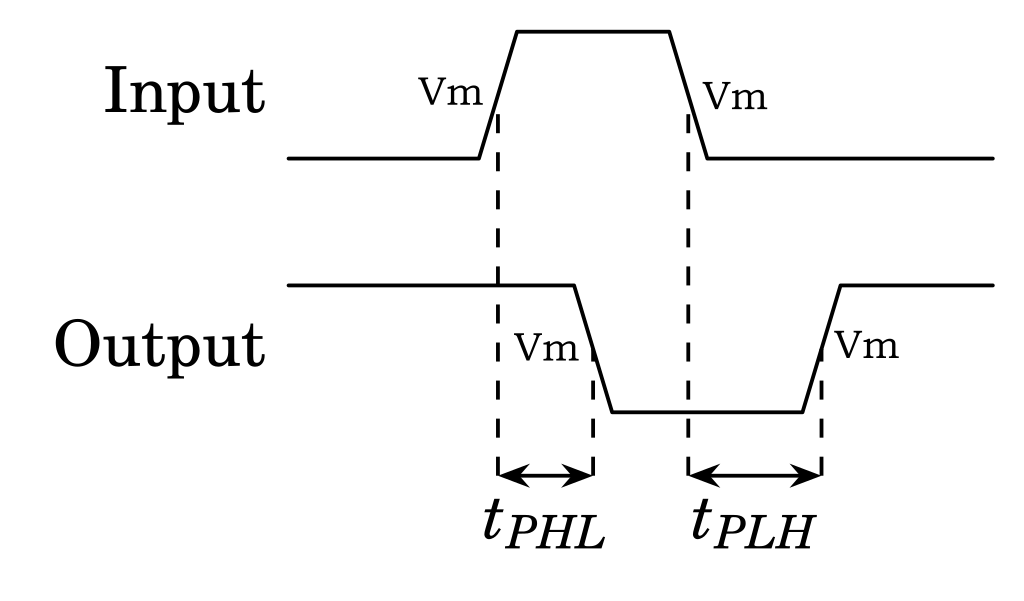
\includegraphics[scale=0.4]{notdelay_mark}
	\caption{Diagramma dei tempi di propagazione per una porta NOT
	\label{fig: notdelay}}
\end{figure}

Prendiamo quindi come definizione di tempo di propagazione il lasso di tempo
che trascorre tra quando $V\ped{in}$ diventa pari a $V\ped{I, med}$ e
$V\ped{out}$ diventa pari al suo $V\ped{O, med}$, dove i valori medi tra stato
basso e stato alto rispettivamente per l'ingresso e per l'uscita sono
definiti intuitivamente dalle formule
\begin{align*}
V\ped{O, med} &= \frac{V_{OH} + V_{OL}}{2} \\
V\ped{I, med} &= \frac{V_{IH} + V_{IL}}{2} \\
\end{align*}

Dal datasheet si ricavano come tempi di propagazione attesi:
\begin{align*}
    t_{PHL,max} &= 22 \; \si{n\s} \\
    t_{PLH,max} &= 15 \; \si{n\s} \\
\end{align*}

\subsection{Misura dei tempi con l'oscillografo}
Come visto anche nella \cref{sec: tens}, inviando in ingresso un'onda quadra
compresa tra 0 e 5 V, all'uscita della porta troviamo la stessa onda compresa
tra $V_{OH} \approx 3.6 \; \si{\V}$ e $V_{OL} \approx 0.3  \; \si{V}$;
infatti misurando con i cursori e con l'oscilloscopio troviamo come
\begin{align*}
V\ped{O, med} = 1.95 \pm 0.02 \\
V\ped{I, med} = 2.50 \pm 0.03 \\
\end{align*}

Quindi, una volta collegati i due canali all'ingresso (CH1) e all'uscita (CH2)
del NOT gate, abbiamo scelto come evento di trigger il passaggio del segnale
di ingresso per $V_{I,med}$, abbiamo dunque cambiato il fronte tra
salita/discesa per scegliere se misurare il tempo di propagazione H->L o L->H.
\begin{figure}[htbp]
\centering
	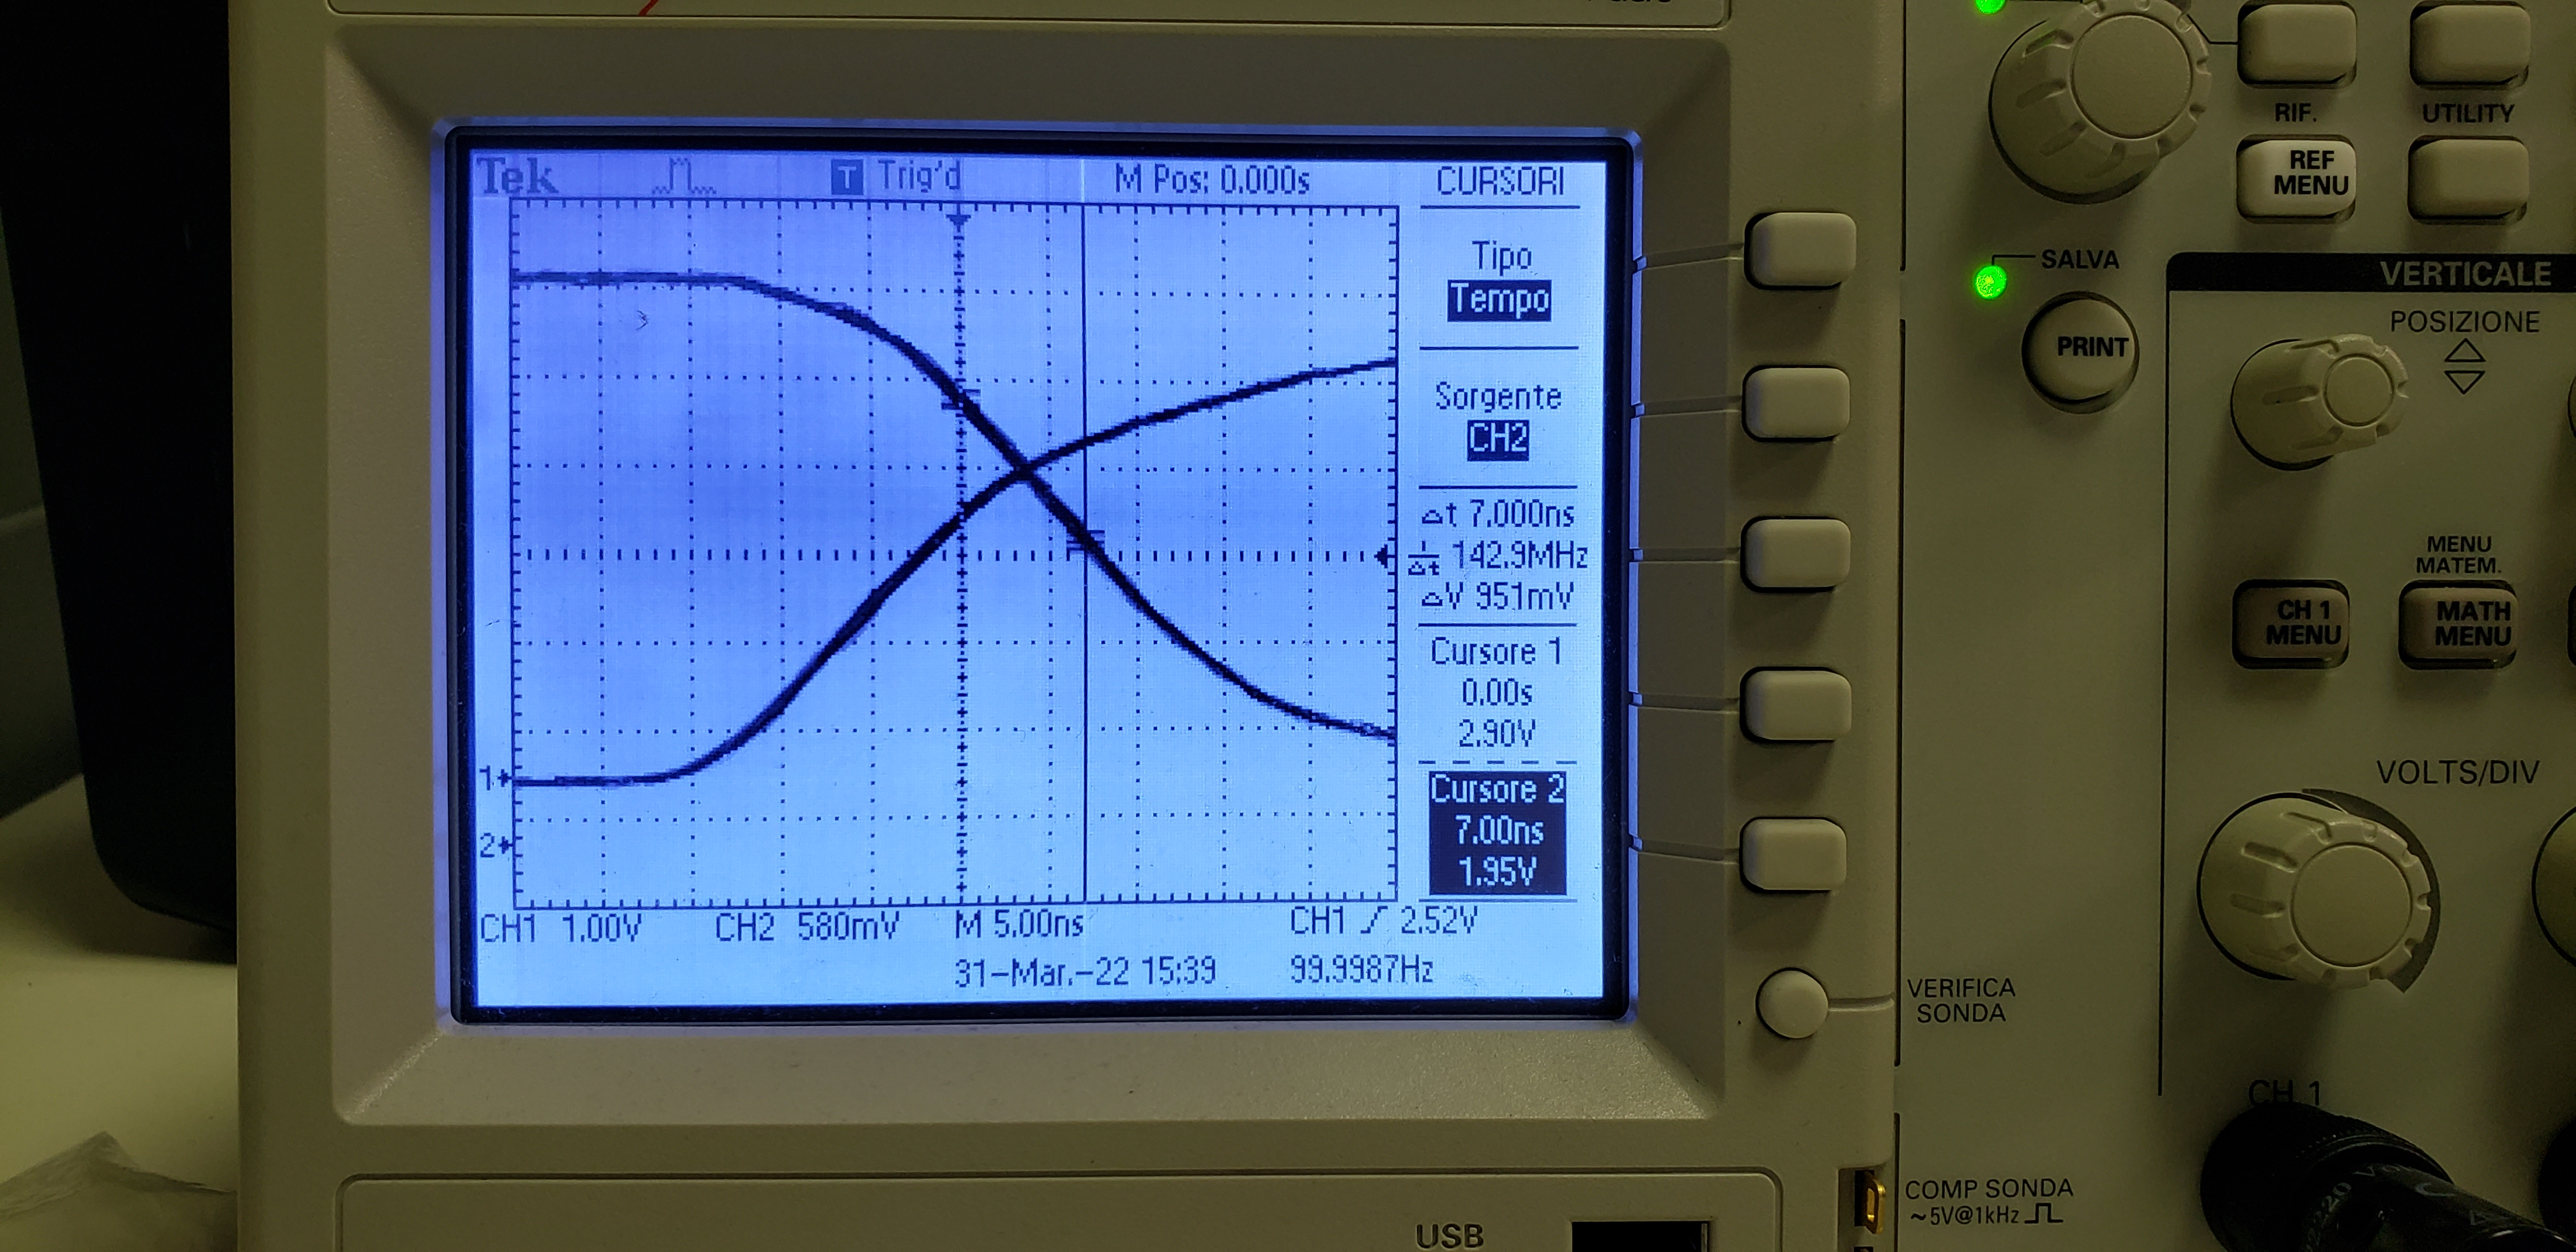
\includegraphics[width=\textwidth]{LH1}
	\caption{Acquisizione tramite oscilloscopio digitale della transizione da
	L a H per il primo integrato}
\end{figure}
\begin{figure}[htbp]
\centering
	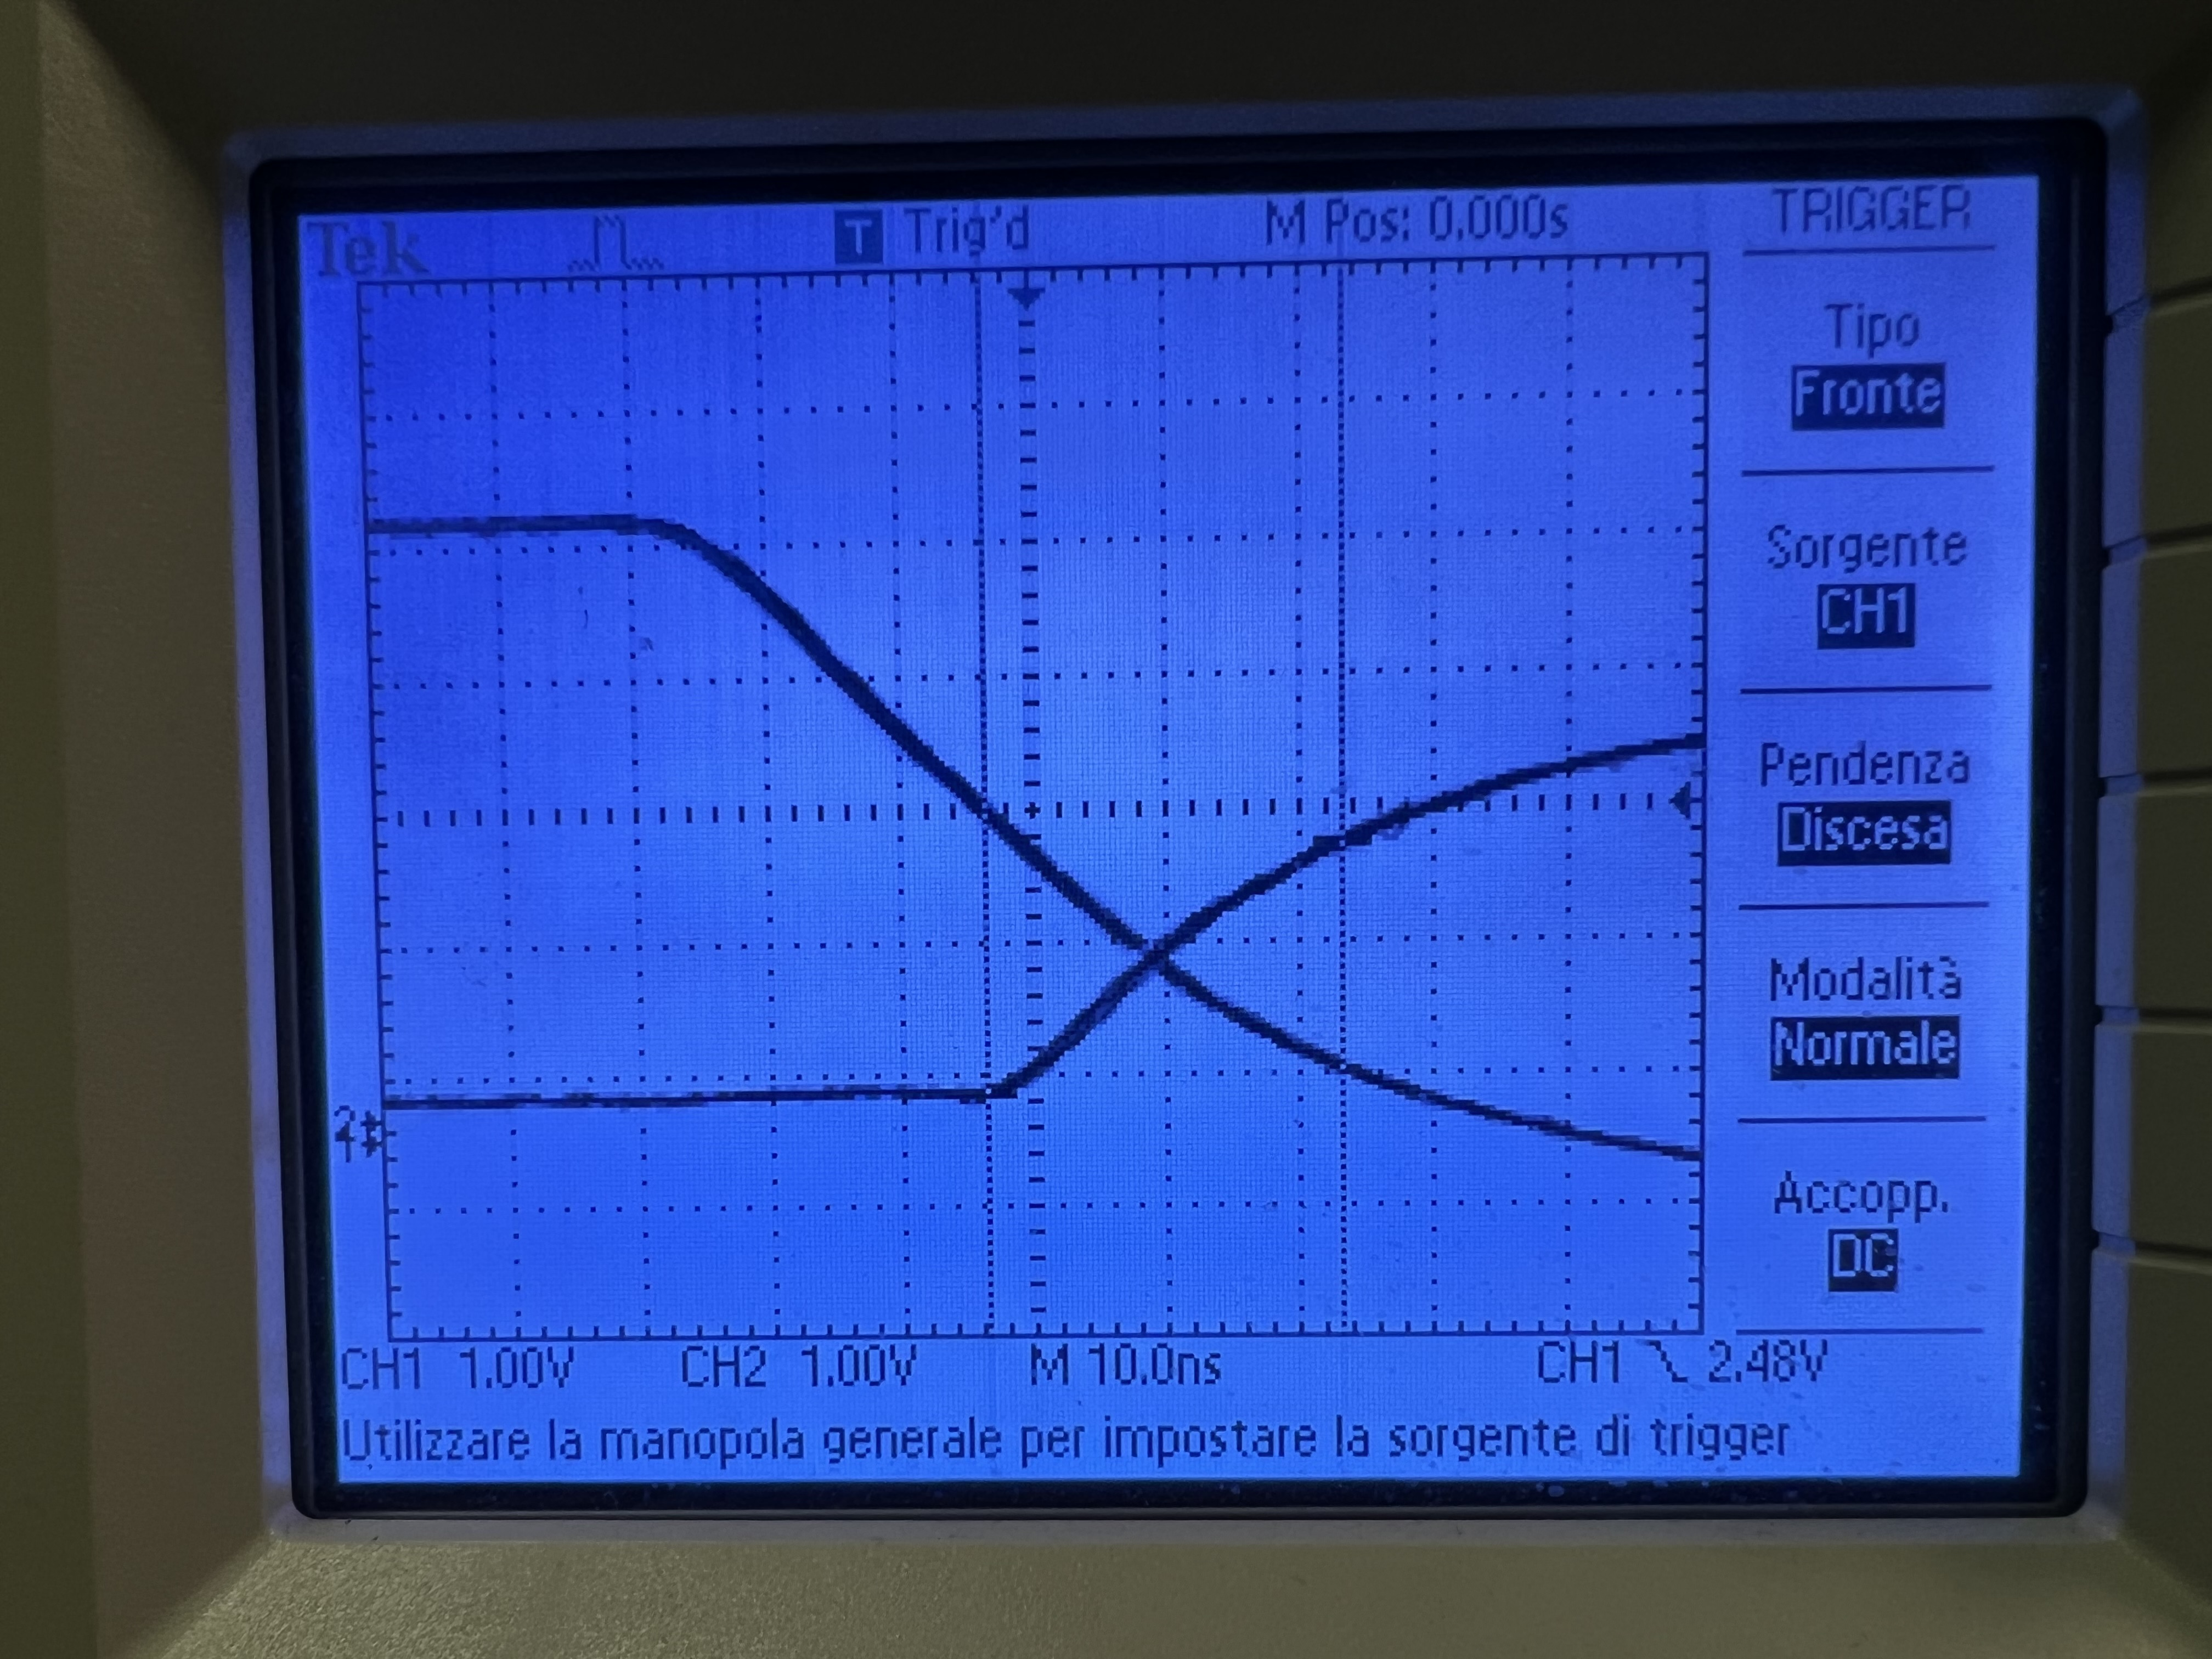
\includegraphics[width=\textwidth]{LH2}
	\caption{Acquisizione tramite oscilloscopio digitale della transizione da
	L a H per il secondo integrato}
\end{figure}
\begin{figure}[htbp]
\centering
	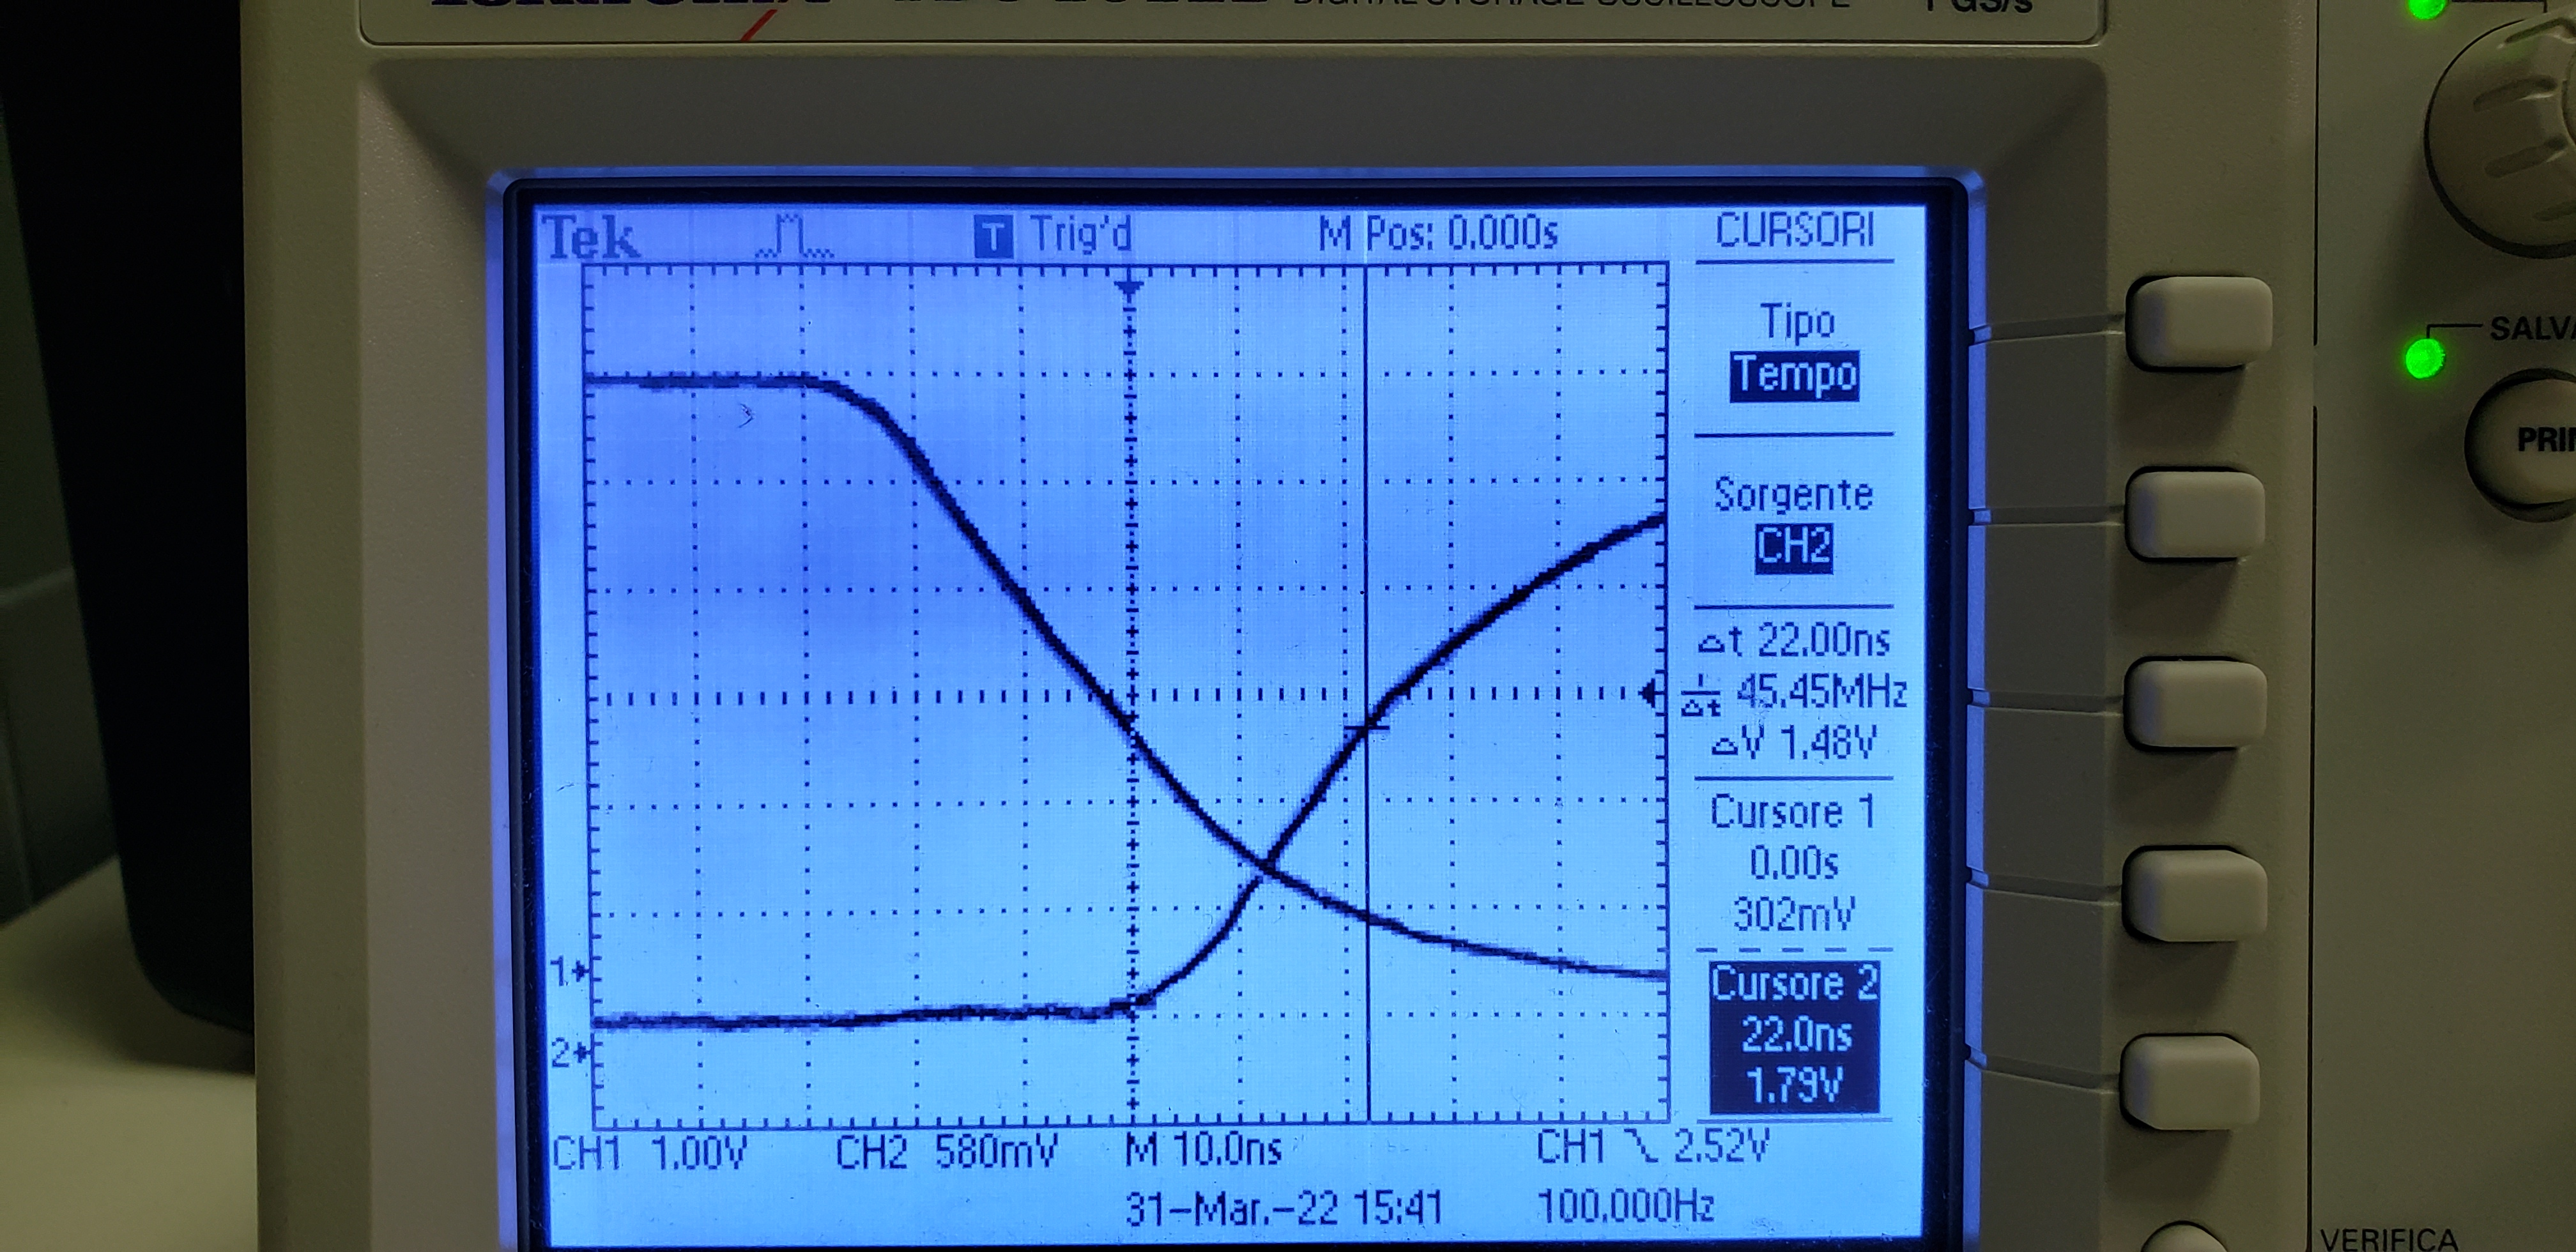
\includegraphics[width=\textwidth]{HL1}
	\caption{Acquisizione tramite oscilloscopio digitale della transizione da
	H a L per il primo integrato}
\end{figure}
\begin{figure}[htbp]
\centering
	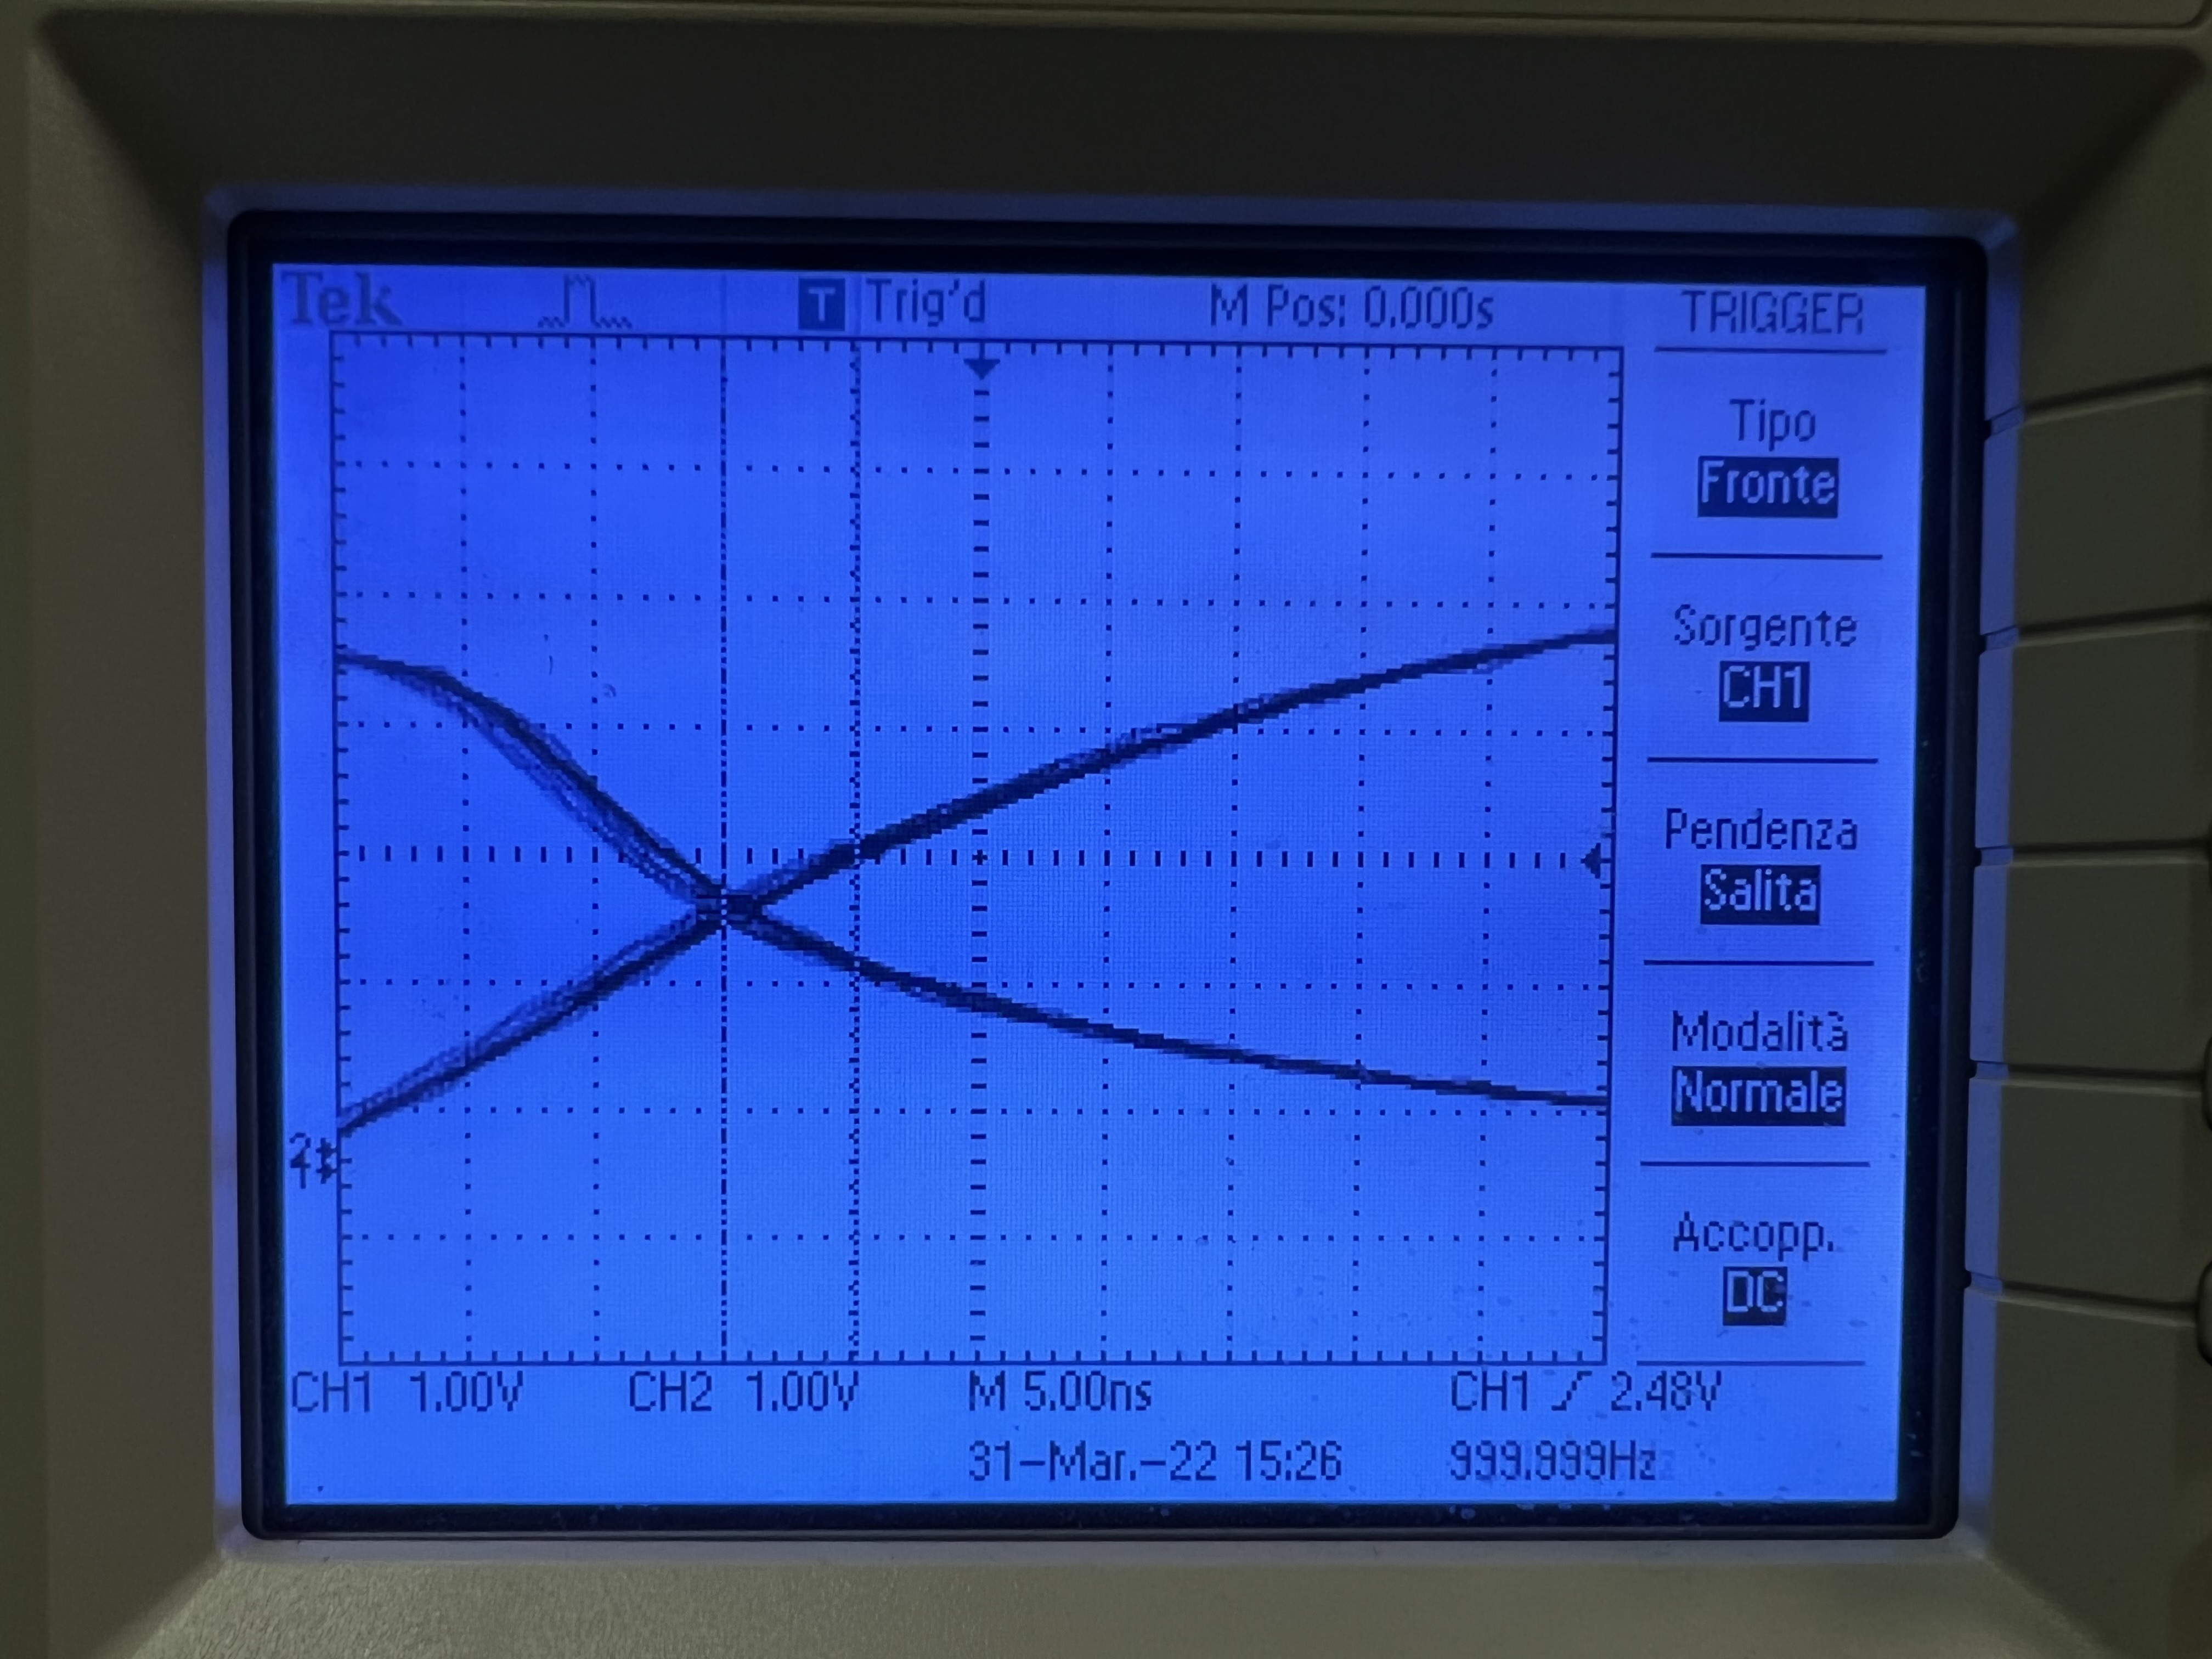
\includegraphics[width=\textwidth]{HL2}
	\caption{Acquisizione tramite oscilloscopio digitale della transizione da
	H a L per il secondo integrato}
\end{figure}

Dalle misure prese con i cursori dell'oscilloscopio (a cui associamo come
incertezza il contributo dato dalle specifiche del datasheet, tenendo conto
dell'instabilità delle tracce sullo schermo) troviamo
\begin{multicols}{2}
    \centering
    $t_{PLH}=$ 5.2 $\pm$ 1.2 \si{n\s} \\
    $t_{PHL}=$ 25 $\pm$ 2 \si{n\s}
    
    $t_{PLH}=$ 7.0 $\pm$ 1.2 \si{n\s} \\
    $t_{PHL}=$ 22 $\pm$ 2 \si{n\s}
\end{multicols}

\subsection{Confronto con i valori attesi}
Le misure dei tempi di propagazione nella transizione basso->alto risultano
compatibili con i valori tipici, quindi sicuramente compresi entro
l'intervallo massimo garantito dal costruttore.

Mentre per quanto riguarda la transizione opposta, abbassando la scala dei
tempi osserviamo che i segnali visualizzati dall'oscilloscopio risultano
simili alle curve caratteristiche di carica e scarica di un condensatore
(riportata in \cref{fig: carica}).
\begin{figure}[htbp]
\centering
	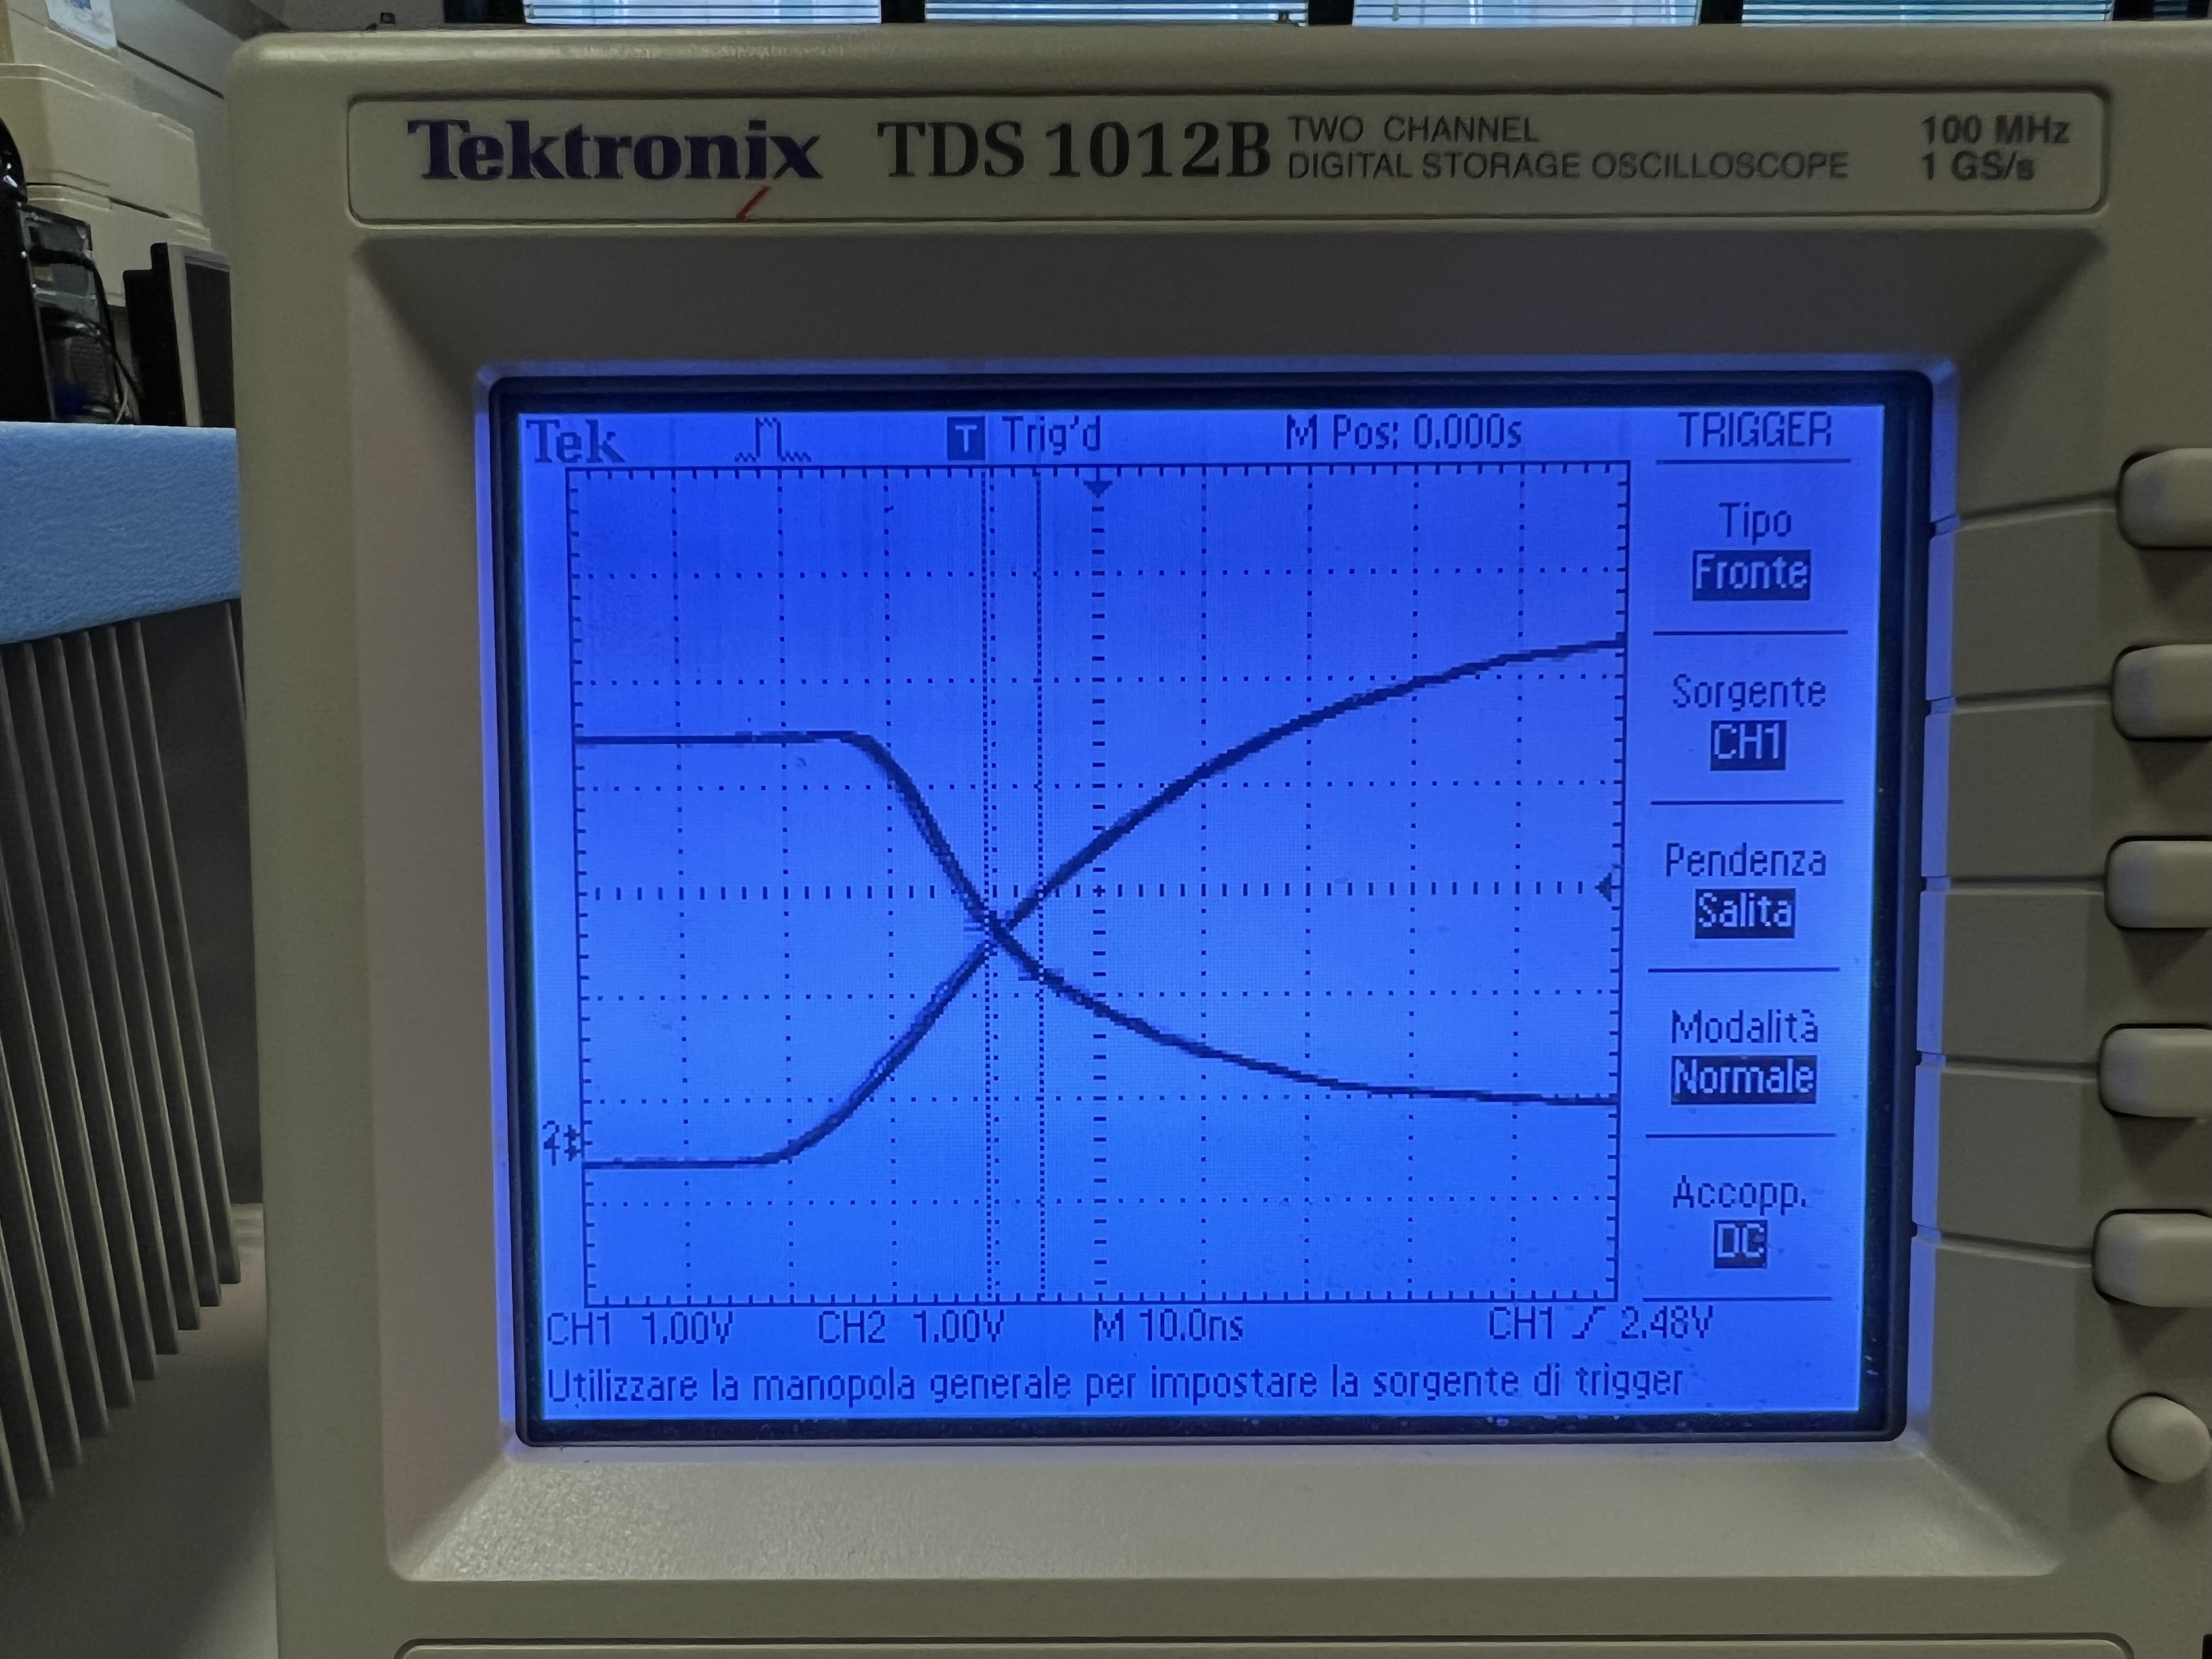
\includegraphics[width=\textwidth]{carica}
	\label{fig: carica}
	\caption{Acquisizione con oscilloscopio digitale con un fondo scala dei tempi più piccolo, in modo da osservare qualitativamente come la propagazione del segnale assomigli molto al grafico della tensione ai capi di un condensatore durante il ciclo di carica/scarica}
\end{figure}

Effettivamente a causa di questa discesa molto lenta del segnale in uscita
abbiamo misurato dei tempi di propagazione $t_{PHL}$ per il primo integrato
al limite massimo riportato nel datasheet e addirittura oltre le specifiche
per il secondo.

Rimane difficile valutare se questo tempo di discesa lungo sia dovuto ad
accoppiamenti capacitivi spuri fra la basetta, i cavi di connessione o interne
agli integrati usati, per cui se la definizione di tempo di propagazione non
risulta ben posta prendiamo le nostre misure come stime indicative dei valori
effettivi, che risultano compatibili con quanto dichiarato nel datasheet con
uno scarto del $14 \; \percent$.

\setcounter{section}{3}
%=======================
\section*{Parte B: Circuiti logici elementari con sole porte NAND}
La caratteristica più fondamentale delle porte NAND è la loro universalità,
infatti è possibile realizzare qualsiasi tipo di circuito logico tramite
combinazione di sole porte NAND (o NOR). In questa parte intendiamo costruire
e verificare il funzionamento di circuiti equivalenti a porte OR, XOR e
multiplexer a partire da soli chip NAND SN74LS00.
\begin{figure}[htbp]
\centering
    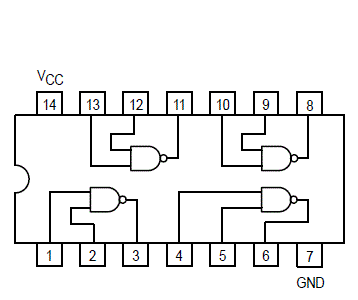
\includegraphics[width=0.3\textwidth]{NAND}
    \caption{Schema e pedinatura del circuito integrato SN74LS00 quad-NAND
    \label{fig: NAND}}
\end{figure}

\section{Tabella di verità}
\subsection{Verifica statica della tabella di verità NAND}
Vogliamo verificare preliminarmente che la porta NAND funzioni correttamente
grazie alla funzione StaticIO inviando a DIO 0 e DIO 1 due segnali di tipo
switch in tutte le loro possibili combinazioni. I primi due canali sono
collegati agli ingresso di una stessa porta NAND sotto, mentre da DIO 2 in
modalità LED misurare il valore in uscita da questa.
\begin{figure}[htbp]
	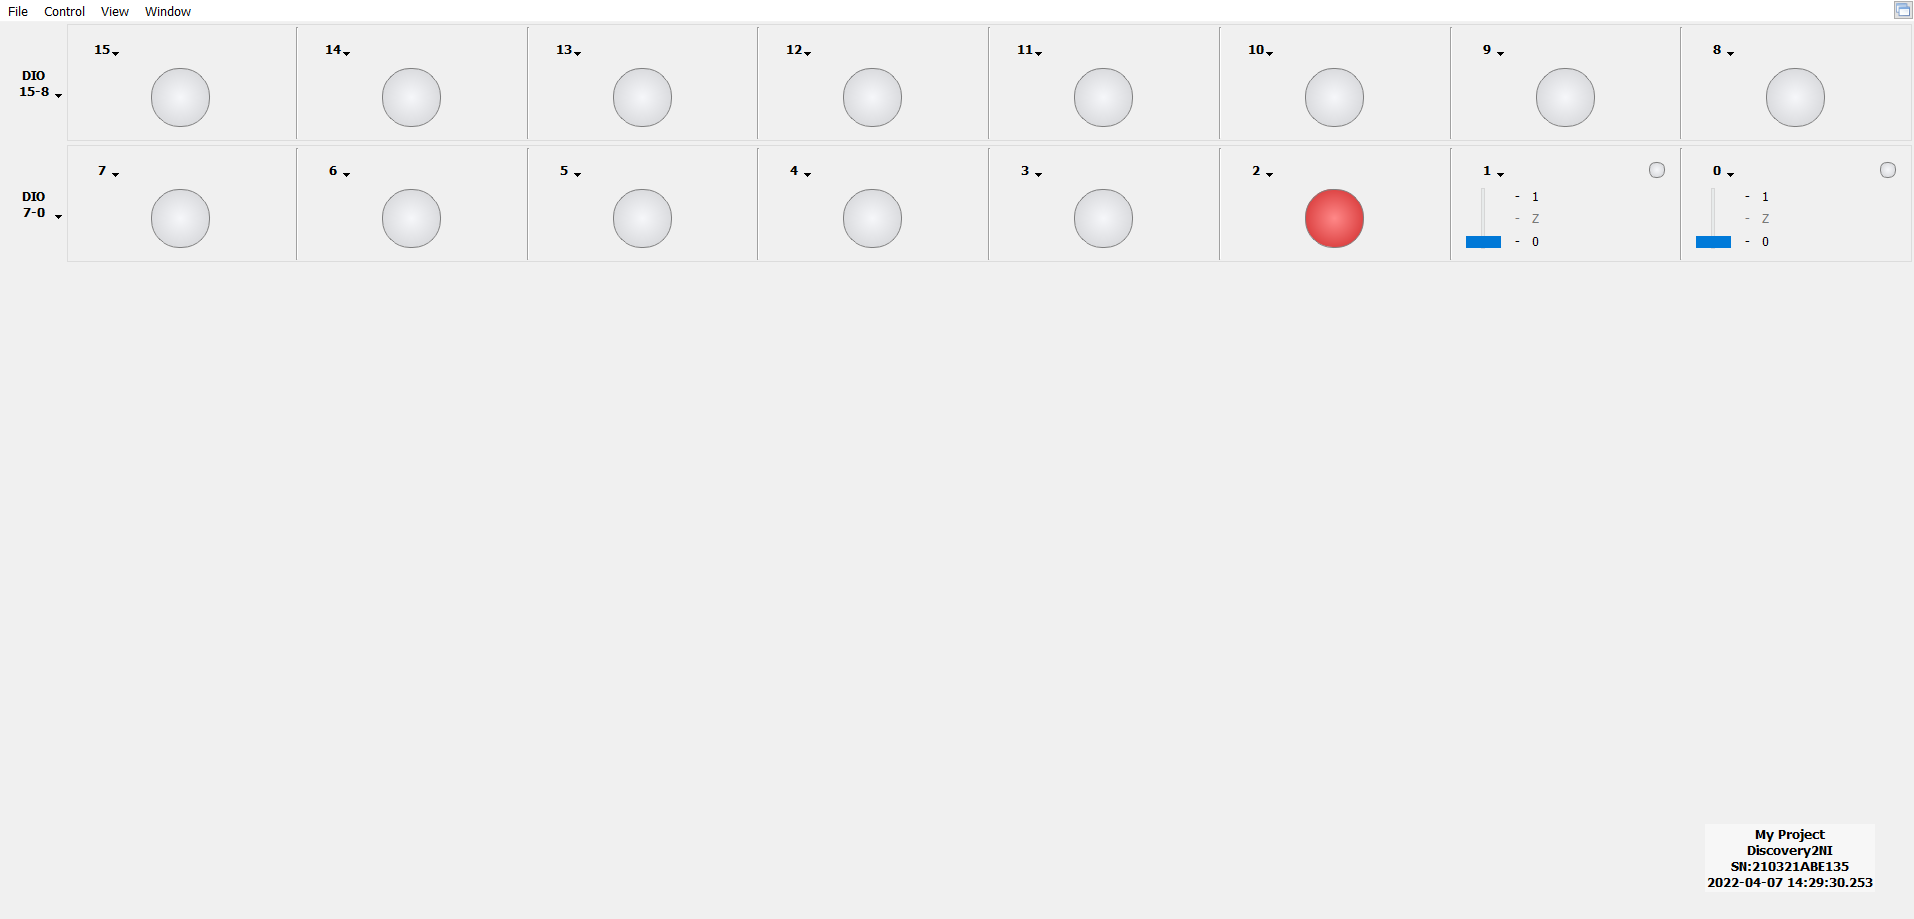
\includegraphics[scale=0.21]{static_nand00}
	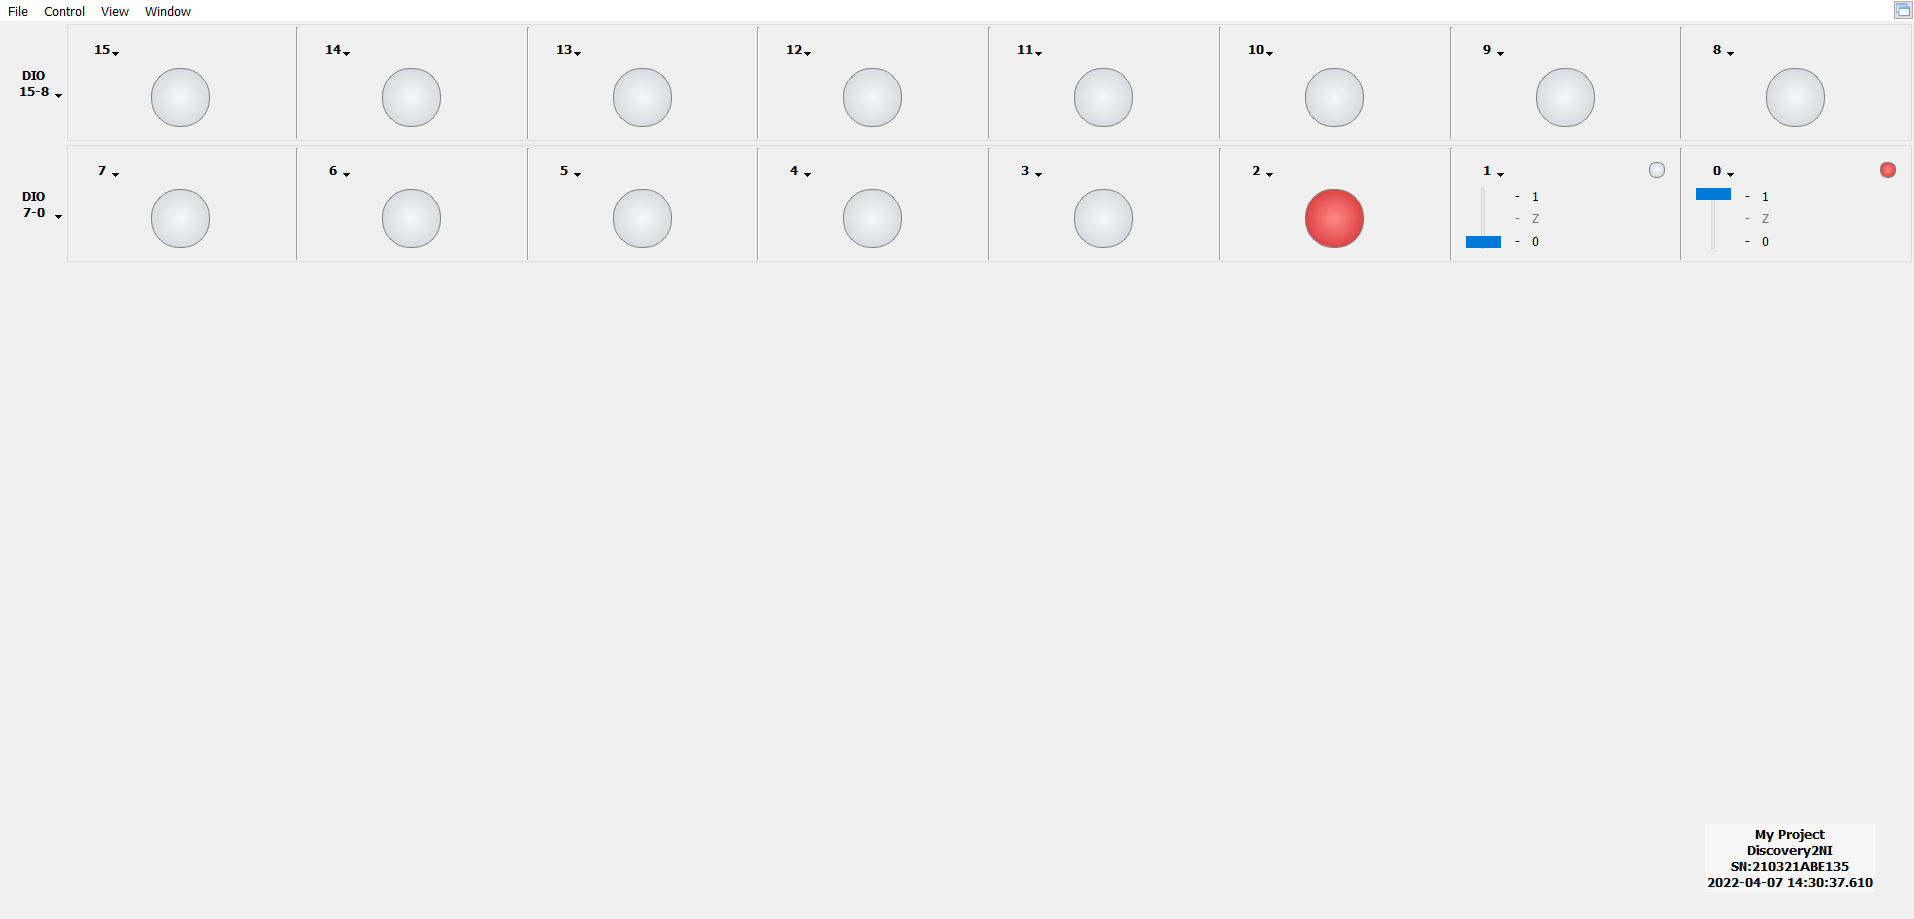
\includegraphics[scale=0.21]{static_nand01}
	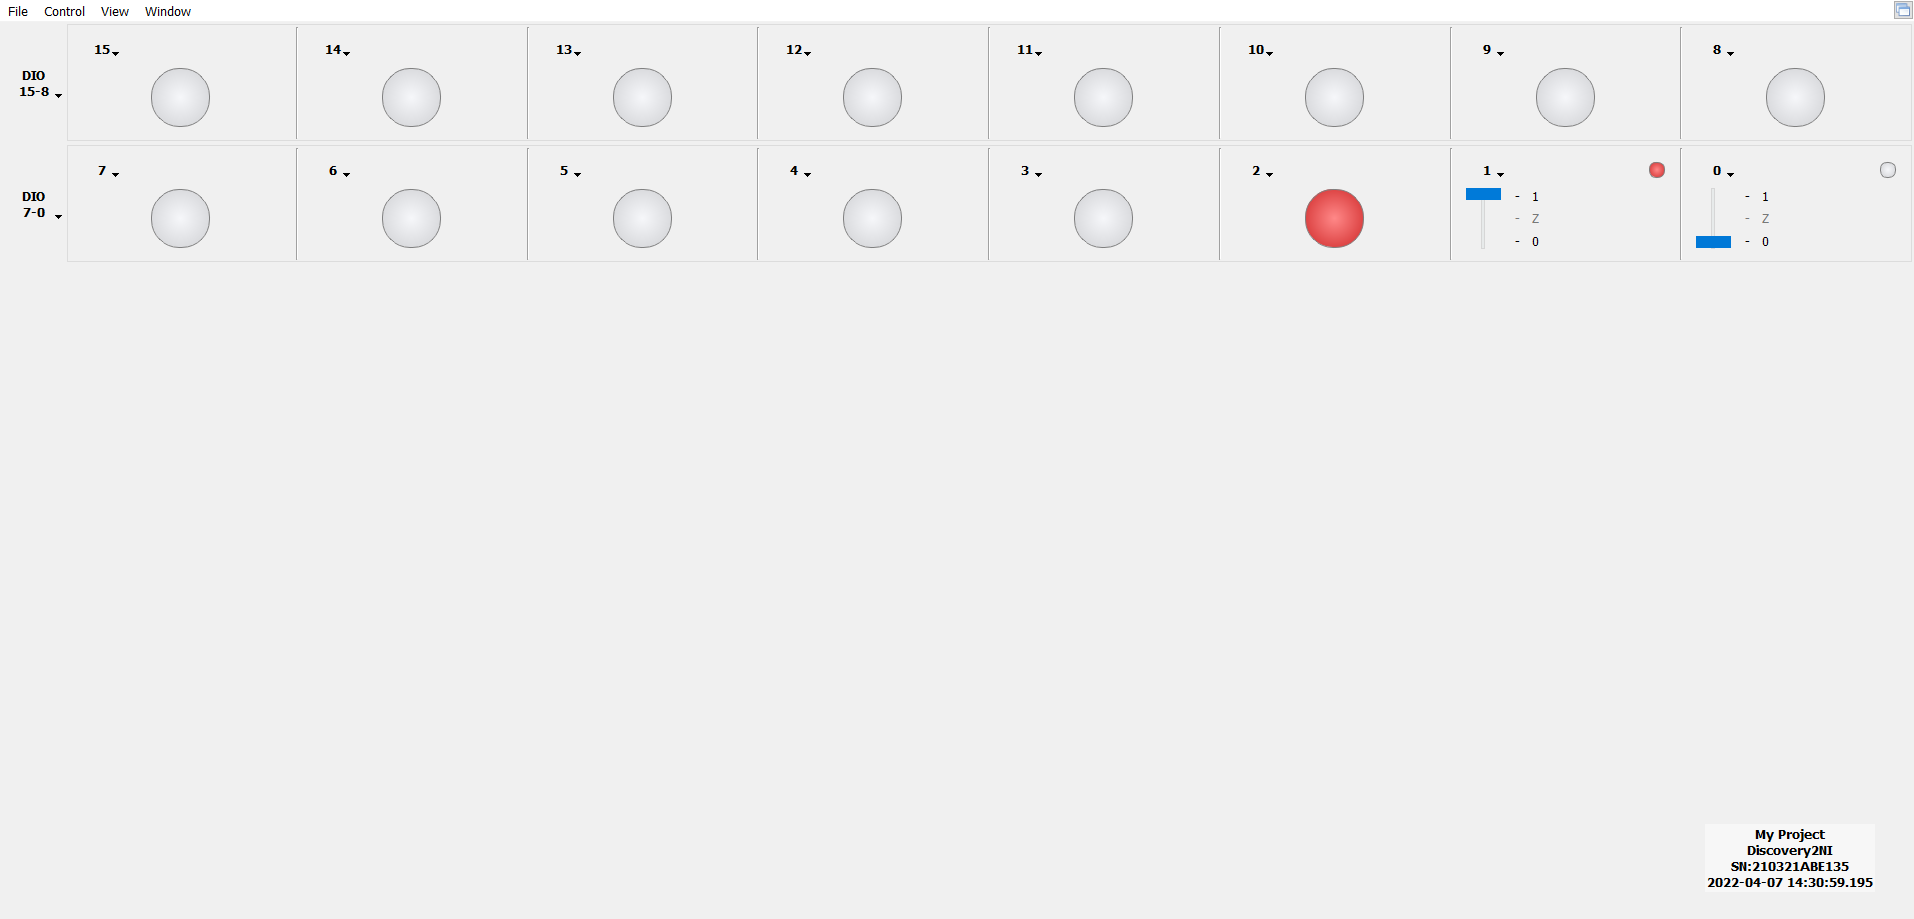
\includegraphics[scale=0.21]{static_nand10}
	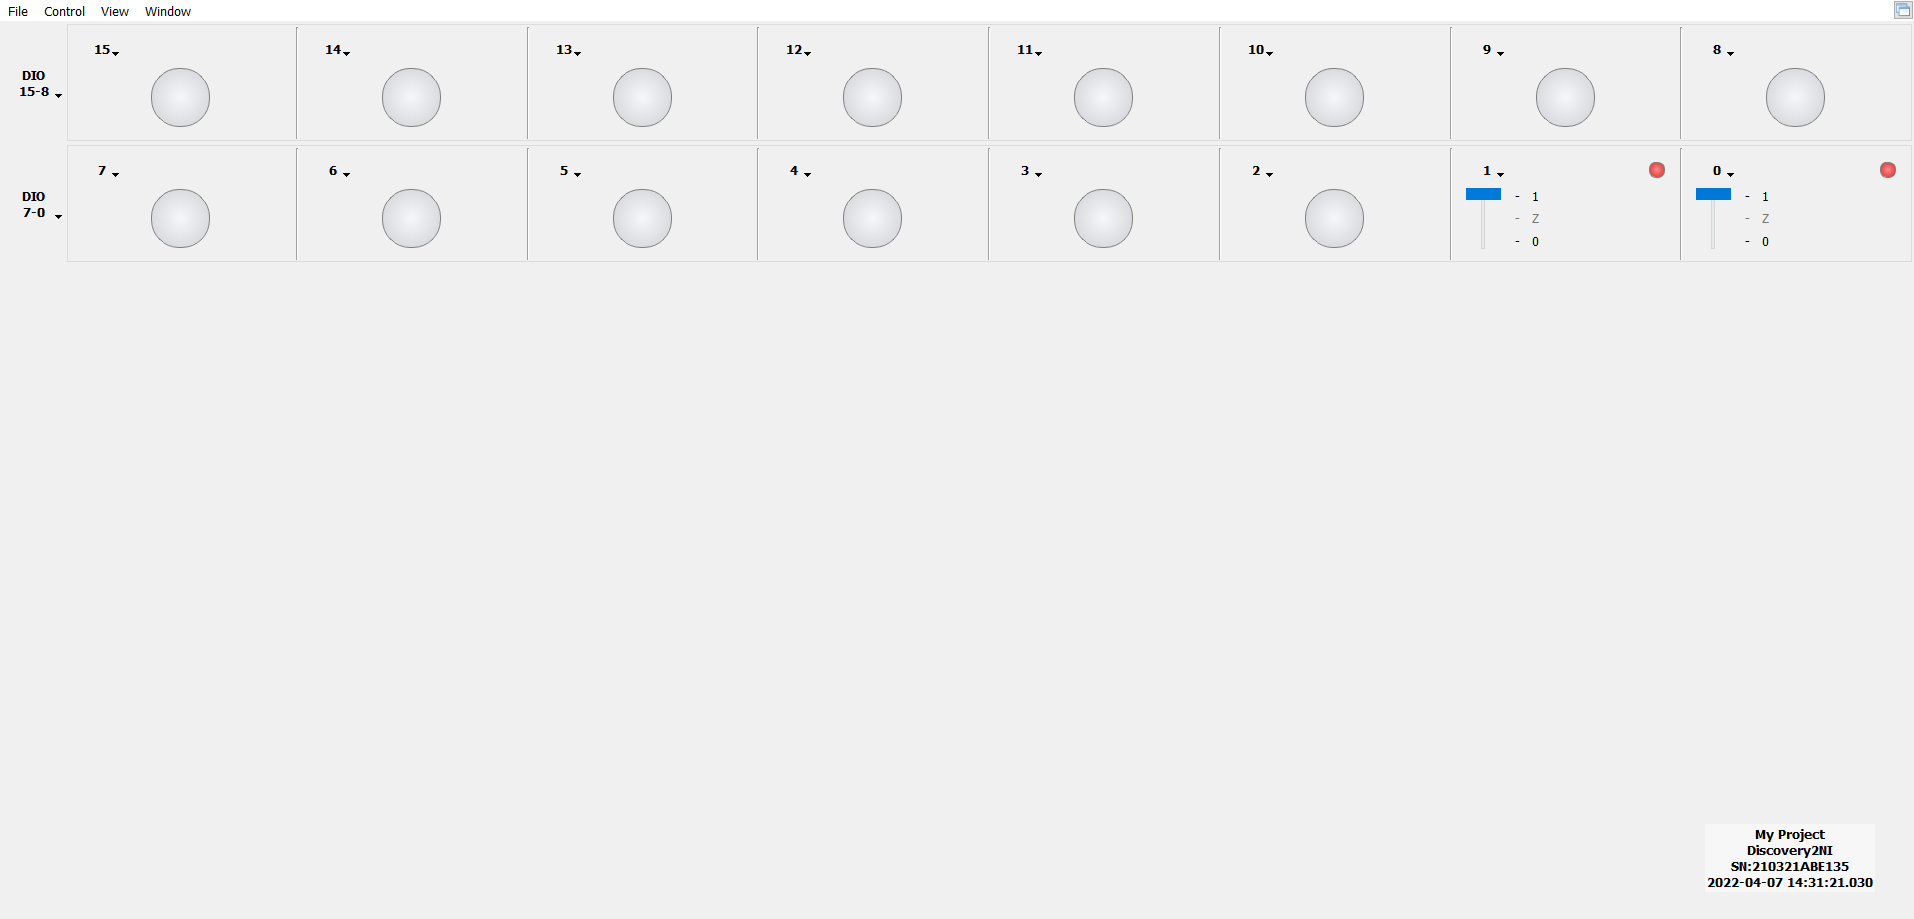
\includegraphics[scale=0.21]{static_nand11}
	\caption{Acquisizione tramite StaticIO delle possibili configurazioni della
	porta NAND, in funzione dei valori di input}
\end{figure}
\subsection{Verifica del funzionamento con Logic Analyzer}
Definiamo dentro lo strumento Patterns (generator) di WaveForms 2 segnali
di clock; uno di frequenza 100 Hz (in uscita dalla porta DIO0) e l'altro a
200 Hz (in uscita dalla porta DIO1) in modo che la loro combinazione produca
tutte le coppie di valori ottenibili con 2 bit.

Dunque si sono pilotati i due ingressi di una stessa porta NAND collegando
i due clock ad un ingresso ciascuno e tramite lo strumento Logic (Analyzer)
si sono acquisiti gli andamenti nel tempo dei due segnali in ingresso e di
quello in uscita dalla porta studiata (riportata in \cref{fig: nand_time})
\begin{figure}[htbp]
\centering
	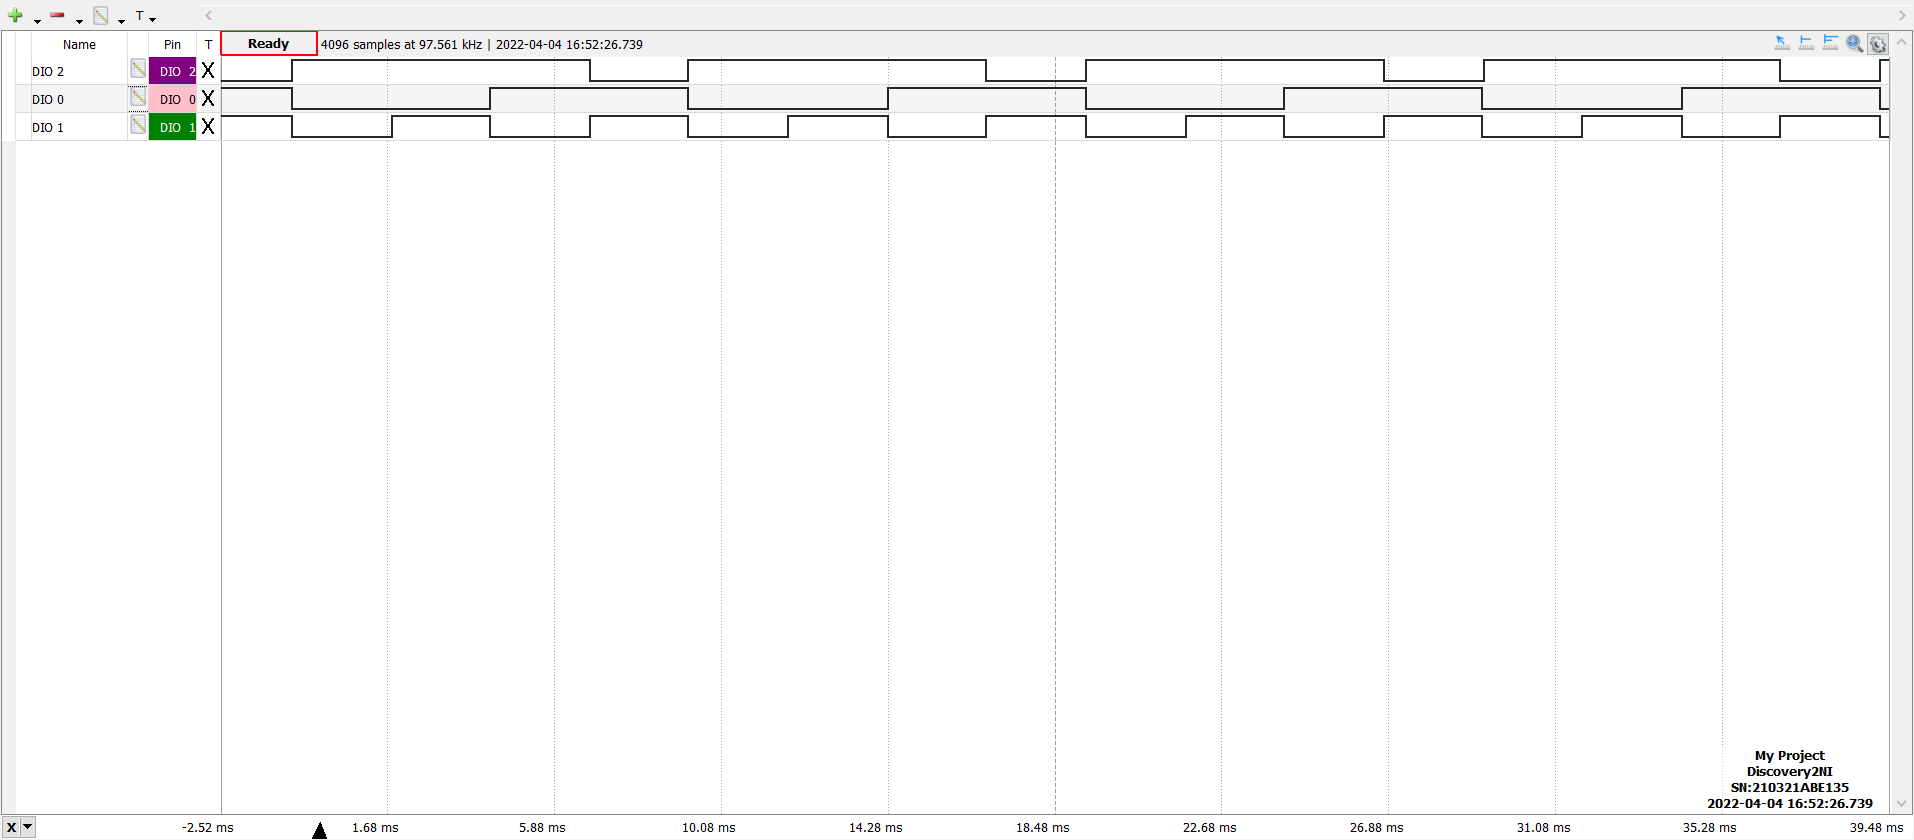
\includegraphics[scale=0.4]{nand_time}
	\caption{Acquisizione di Logic di una porta NAND guidata da due segnali da
	DIO0 (100 Hz) e DIO1 (200 Hz); in uscita viene letto da DIO2}
	\label{fig: nand_time}
\end{figure}
Il circuito risulta essere funzionante e l'output risulta essere L se e solo
se i pin 1 e 2 valgono entrambi H, proprio come da aspettative.

\section{Costruzione di circuiti con porte NAND}
\subsection{Porta OR}
Come primo circuito si costruisce una porta OR: detti $A$ e $B$ gli ingressi
e $Y$ l'uscita, la funzione OR nella notazione dell'algebra di Boole si
indica come
\[
Y = A + B
\]
Sfruttando la legge di De Morgan si ottiene la stessa relazione in termini
di operatori NAND:
\begin{equation}
    Y = A + B = \overline{\overline{A}\cdot\overline{B}}
\end{equation}

Sapendo che per ottenere un NOT basta collegare lo stesso ingresso a un NAND
gate, si può disegnare lo schema logico del circuito come in
\cref{fig: OR_tikz}:
\begin{figure}[htbp]
    \centering
    \begin{circuitikz}
        \draw (0,0) node (nand) [nand port] {};
        \draw (nand.in 1) ++(-0.5, 0) node (not1) [not port, scale=0.4] {};
        \draw (nand.in 2) ++(-0.5, 0) node (not2) [not port, scale=0.4] {};
        \draw (not1.out) -- (nand.in 1);
        \draw (not2.out) -- (nand.in 2);
        \draw (not1.in) -- ++(-0.5, 0) node[anchor=east] {$ A $};
        \draw (not2.in) -- ++(-0.5, 0) node[anchor=east] {$ B $};
        \node[anchor=west] at (nand.out) {$ A + B $};
    \end{circuitikz}
    \caption{\label{fig: OR_tikz}}
\end{figure}

Che corrisponde nella nostra implementazione reale con l'integrato SN74LS00
allo schema circuitale in \cref{fig: OR_circ}.
\begin{figure}[htbp]
    \centering
    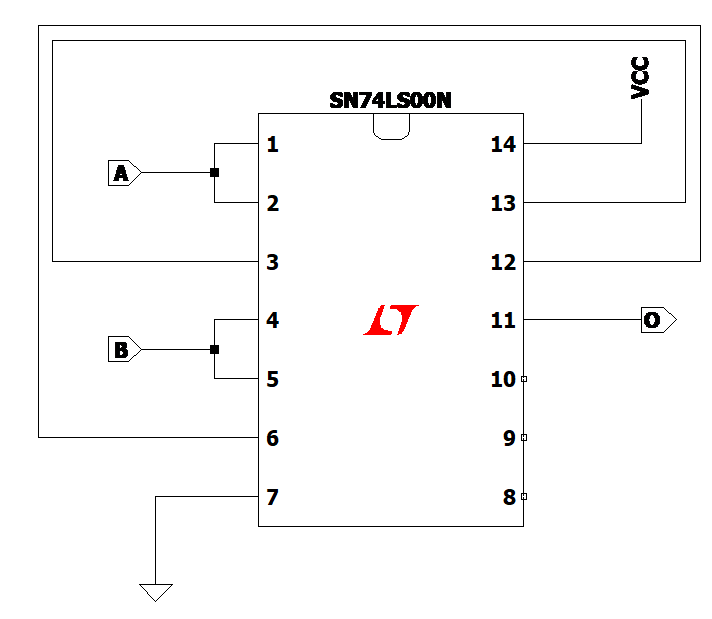
\includegraphics[width=0.45\textwidth]{NAND_OR}
    \caption{Schema circuitale utilizzato per costruire un
    OR GATE: $A$ e $B$ sono i segnali di input, mentre $O \equiv Y$ qui è
    l'output \label{fig: OR_circ}}
\end{figure}

Utilizzando le funzioni Patterns e Logic abbiamo inviato dai pin DIO0 e DIO1
2 segnali di clock di frequenza 50 e 100 Hz e abbiamo utilizzato la porta
DIO2 per verificare che l'output del circuito combaciasse con i valori attesi
dalla tabella di verità della funzione logica OR (come si vede in
\cref{fig: or_time})
\begin{figure}[htbp]
    \centering
    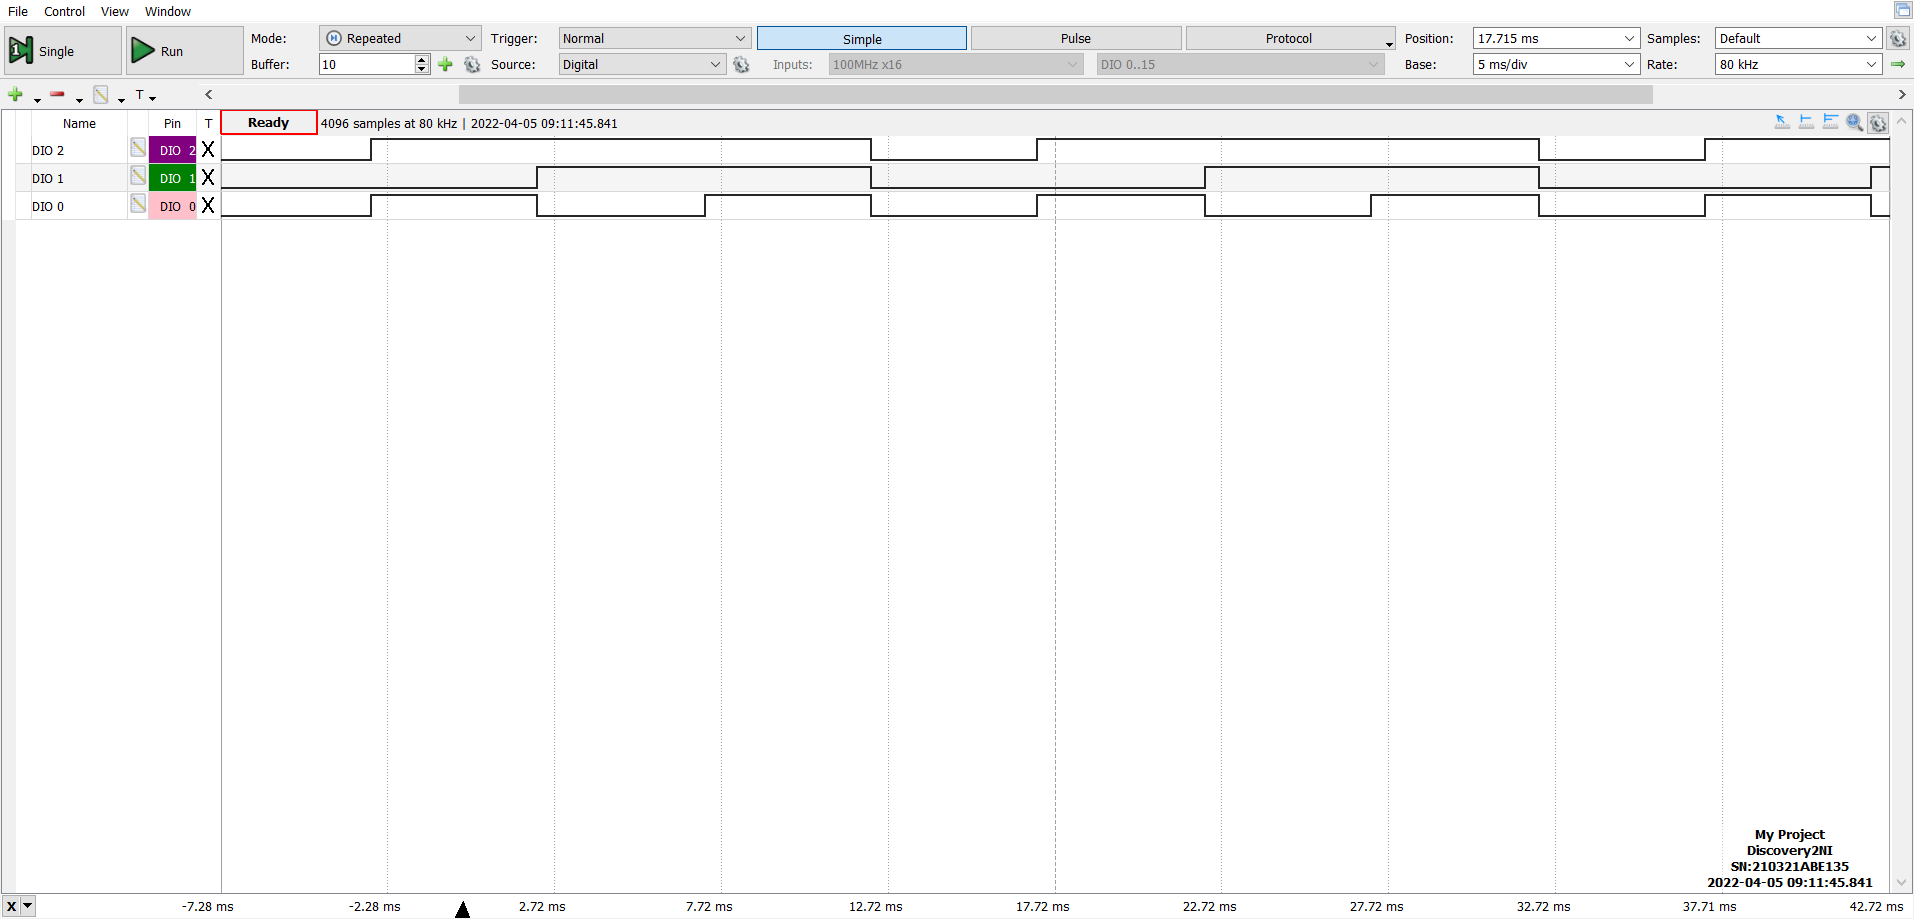
\includegraphics[width=\textwidth]{or_time}
    \caption{Acquisizione di Logic per il circuito OR costruito tramite NAND: DIO0 e DIO1 sono i segnali in input, DIO2 è l'output\label{fig: or_time}}
\end{figure}
Si vede quindi che il circuito ha il funzionamento aspettato con l'output L se e solo se i due input sono entrambi L.

\subsection{Circuito selettore a due vie (multiplexer)}
Realizziamo un circuito che permetta di assegnare all'uscita il valore di
uno dei due ingressi a singolo bit tramite il valore di un terzo ingresso.
Indichiamo con $A$, $B$ e $C$ gli ingressi e con $Y$ l'uscita.
In notazione logica il circuito implementa la funzione
\[
    \begin{cases}
    C = 0 \implies Y = A \\
    C = 1 \implies Y = B
    \end{cases}
\]
che corrisponde alla mappa di Karnaugh riportata in \cref{tab: mult_map} e alla
tabella di verità scritta in forma esplicita in \cref{tab: mult_ver}
\begin{table}
    \centering
    \begin{tabular}{c||c|c|c|c}
        \backslashbox{C}{AB} & 00 & 01 & 11 & 10\\
        \hline
        \hline
        0 & 0 & 0 & 1 & 1\\
        \hline
        1 & 0 & 1 & 1 & 0\\
    \end{tabular}
\caption{Mappa di Karnaugh per un circuito selettore a due vie
\label{tab: mult_map}}    
\end{table}

\begin{table}[htbp]
\centering
\begin{tabular}{ccc|c}
\toprule
$C$ & $A$ & $B$ & $Y$ \\
\midrule
\midrule
0&0&0&0\\
0&0&1&0\\
0&1&0&1\\
0&1&1&1\\
1&0&1&0\\
1&1&0&0\\
1&1&1&1\\
\bottomrule
\end{tabular}
\caption{Tabella di verità del circuito selettore a due vie
\label{tab: mult_ver}}
\end{table}

Da queste possiamo ricavare che l'uscita del circuito deve soddisfare
la relazione
\begin{equation}\label{eq: mult}
Y = A \cdot \overline{C} + B \cdot C
\end{equation}
sempre con la legge di De Morgan si arriva ad una riscrittura dell'
\cref{eq: mult} in termini di NAND
\[
Y = A\cdot\overline{C} + B\cdot C = \overline{(\overline{A\cdot\overline{C}})\cdot(\overline{B\cdot C})}
\]

Che si traduce nello schema logico e nell'implementazione reale del circuito
riportate in \cref{fig: mult_tikz} e \cref{fig: mult_circ} rispettivamente
\begin{figure}[htbp]
    \centering
    \begin{circuitikz}
        \draw (0, 1) node (nandSopra) [nand port] {};
        \draw (0, -1) node (nandSotto) [nand port] {};
        \draw (3, 0) node (nandDestra) [nand port] {};

        \draw (nandSopra.in 2) ++(-0.5,0) node (not) [not port, scale=0.5] {};
        \draw (nandDestra.out) node [anchor=west] {$ \text{SW}(C; A, B) $};
        \draw (nandSopra.in 1) -- ++(-2, 0) node[anchor=east] (input) {$ A $};
        \draw (nandSotto.in 2) -- ++(-2, 0) node[anchor=east] {$ B $};

        \draw (not.out) -- (nandSopra.in 2);
        \coordinate (biforcazione) at ($ (not.out |-, 0) + (-1, 0) $);
        \draw (input |-, 0) node[anchor=east] {$ C $} -- (biforcazione) |- (not.in);
        \draw (biforcazione) |- (nandSotto.in 1);

        \draw (nandSopra.out) -| ++(0.5,0) |- (nandDestra.in 1);
        \draw (nandSotto.out) -| ++(0.5,0) |- (nandDestra.in 2);
    \end{circuitikz}
    \caption{Diagramma logico del circuito selettore
    \label{fig: mult_tikz}}
\end{figure}

\begin{figure}[htbp]
    \centering
    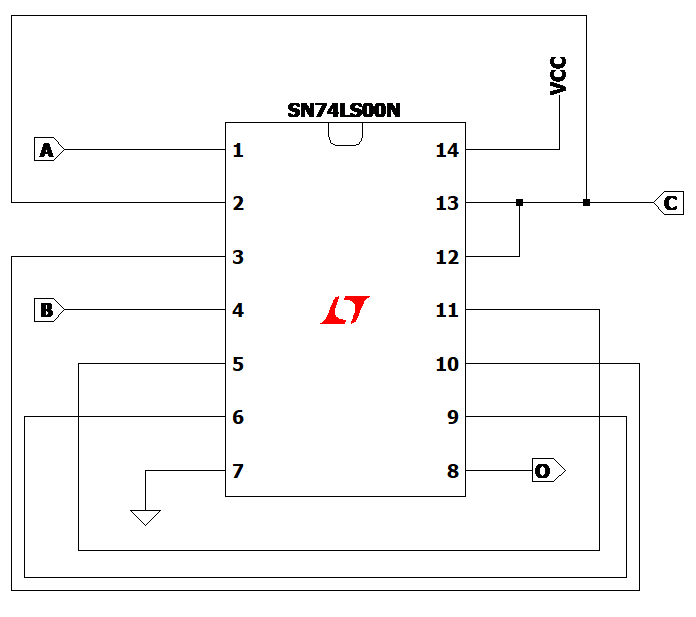
\includegraphics[width=0.6\textwidth]{NAND_MP.png}
    \caption{Schema circuitale di un multiplexer a 2 input, controllato dal
    valore logico di switch $C$}
    \label{fig: mult_circ}
\end{figure}

Per dimostrare il corretto funzionamento del circuito riportiamo la schermata
di configurazione di Patterns, in cui si vede come sono stati impostati gli
ingressi e l'acquisizione di Logic, da cui si può verificare il corretto
funzionamento in uscita dal circuito al variare dei valori logici dei 3
ingressi.

Si inviano all'ingresso del circuito un segnale di clock di frequenza 100 Hz
($B$), uno a 50 Hz $A$ e infine uno a 25 Hz $C$ per esplorare tutte le
possibili combinazioni possibili per i 3 bit di ingresso
(cfr. \cref{fig: mult_pat}).
\begin{figure}[htbp]
    \centering
    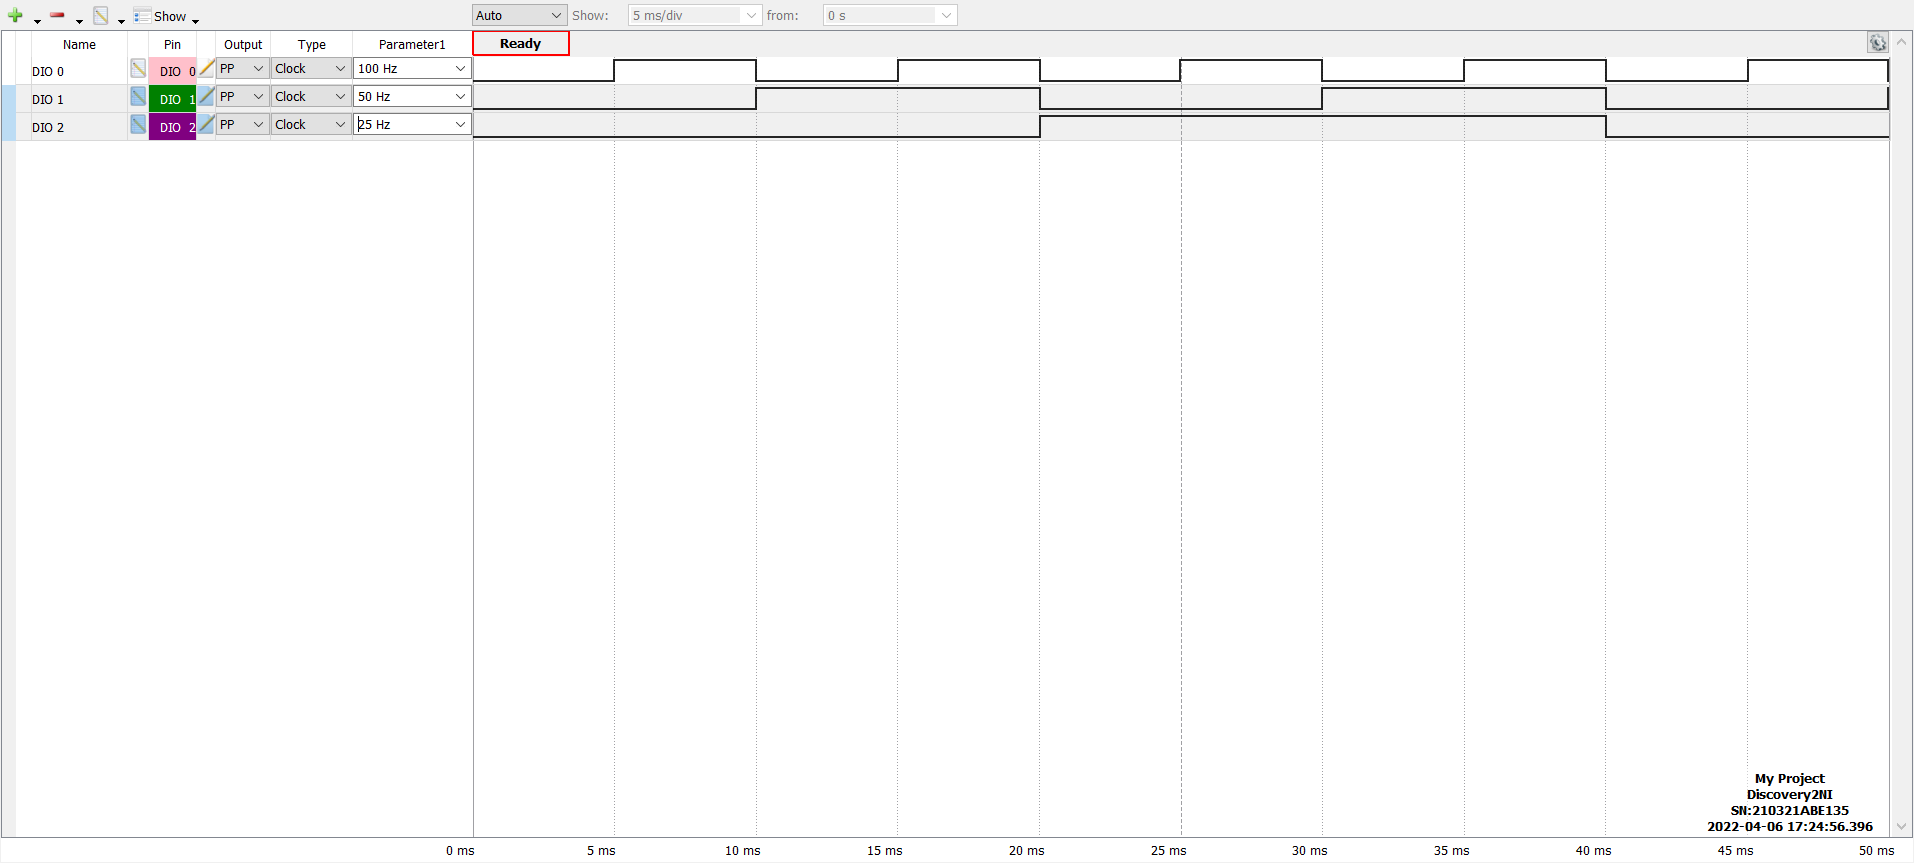
\includegraphics[width=0.8\textwidth]{pat2.png}
    \caption{Schermata di configurazione degli ingressi in Patterns
    al multiplexer: DIO 0 $\equiv B$, DIO 1 $\equiv A$, DIO 2 $\equiv C$.
    \label{fig: mult_pat}}
\end{figure}
\begin{figure}[htbp]
    \centering
    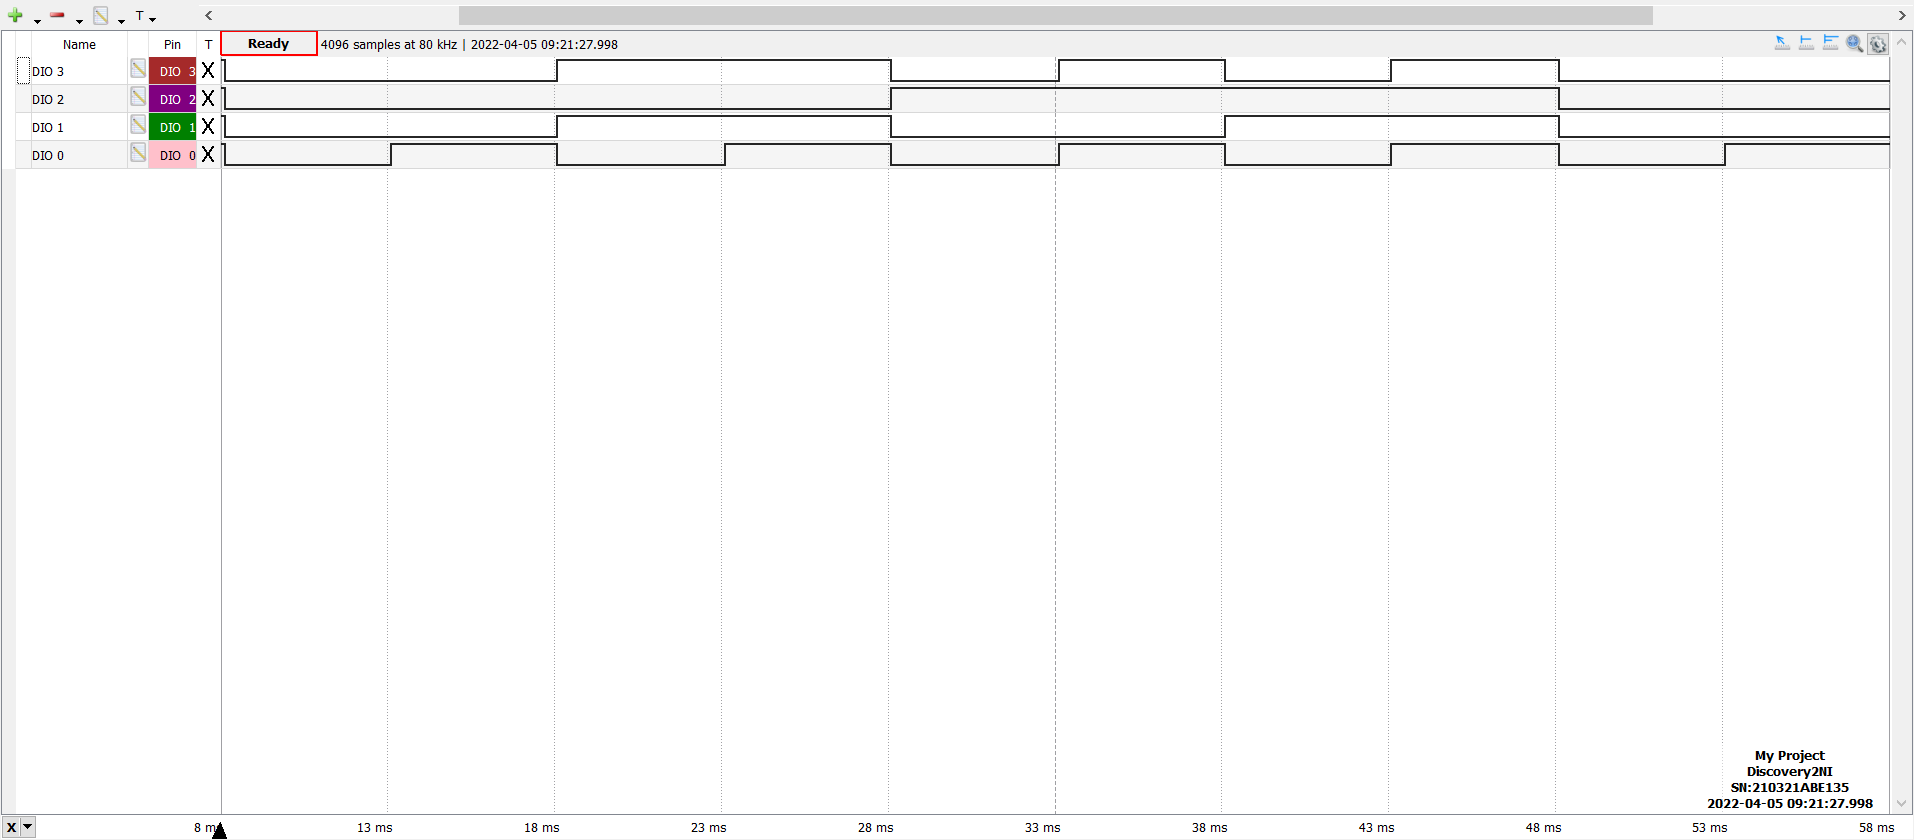
\includegraphics[width=0.8\textwidth]{Multiplex.png}
    \caption{Acquisizione di Logic per il multiplexer: DIO 0 $\equiv B$,
    DIO 1 $\equiv A$, DIO 2 $\equiv C$, DIO 3 $\equiv Y$.}
    \label{fig: mult_log}
\end{figure}
Osserviamo (da \cref{fig: mult_log}) che il circuito funziona come da
aspettative, restituendo cioè il segnale in $A$ nel caso in cui $C = 0$ e
il valore di $B$ quando $C = 1$.

\subsection{Porta XOR}
Un circuito XOR si può realizzare in maniera ottimale con 4 porte NAND
partendo dalla sua equazione caratteristica e manipolandola con le leggi di
De Morgan:
\begin{align*}
  A \oplus B &= (A \cdot \overline{B}) + (\overline{A} \cdot B) = 
 (A \cdot \overline{A} + A \cdot \overline{B}) + (B \cdot \overline{B} +
 \overline{A} \cdot B) \\
 &= A \cdot (\overline{A} + \overline{B}) + B \cdot (\overline{B} +
 \overline{A}) = A \cdot \overline{(A \cdot B)} +
 B \cdot \overline{(B \cdot A)} \\
 &= \overline{\overline{A \cdot \overline{(A \cdot B)}} \cdot
 \overline{B \cdot \overline{(B \cdot A)}}}
\end{align*}

Questo corrisponde allo schema logico e all'implementazione reale con il
nostro chip riportate nelle \cref{fig: XOR_tikz} e \cref{fig: XOR_circ}.
\begin{figure}[htbp]
    \centering
    \begin{circuitikz}
        \draw (0, 1) node (nandSopra) [nand port] {};
        \draw (0, -1) node (nandSotto) [nand port] {};
        \draw (3, 0) node (nandDestra) [nand port] {};
        \draw (-3, 0) node (nandSinistra) [nand port] {};

        \coordinate (biforcazione) at ($ (nandSinistra.out |-, 0) + (0.5, 0) $);
        \draw (nandSinistra.out) -- (biforcazione) |- (nandSopra.in 2);
        \draw (nandSinistra.out) -- (biforcazione) |- (nandSotto.in 1);

        \draw (nandSopra.out) -- ++(0.5,0) |- (nandDestra.in 1);
        \draw (nandSotto.out) -- ++(0.5,0) |- (nandDestra.in 2);
        \draw (nandDestra.out) node [anchor=west] {$ A \oplus B $};
        \draw (nandSopra.in 1) -- ++(-4, 0) node[anchor=east] (inputA) {$ A $};
        \draw (nandSotto.in 2) -- ++(-4, 0) node[anchor=east] (inputB) {$ B $};

        \draw (nandSinistra.in 1) -| (-4.7, |- inputA);
        \draw (nandSinistra.in 2) -| (-4.7, |- inputB);
    \end{circuitikz}
    \caption{Circuito logico di una porta XOR costruita
    con sole porte NAND \label{fig: XOR_tikz}}
\end{figure}

\begin{figure}[htbp]
    \centering
    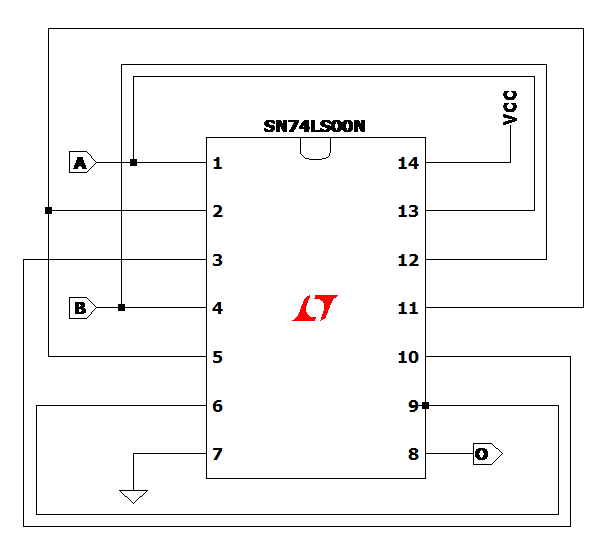
\includegraphics[width=0.6\textwidth]{NAND_XOR}
    \caption{Schema circuitale utilizzato per costruire uno XOR GATE tramite NAND}
    \label{fig: XOR_circ}
\end{figure}

Verifichiamo il buon funzionamento del circuito XOR inviando ai due
ingressi gli stessi segnali di clock usati per la porta OR e osservando i
valori dell'uscita $Y$ con il Logic Analyzer in maniera del tutto analoga a
prima.
\begin{figure}[htbp]
    \centering
    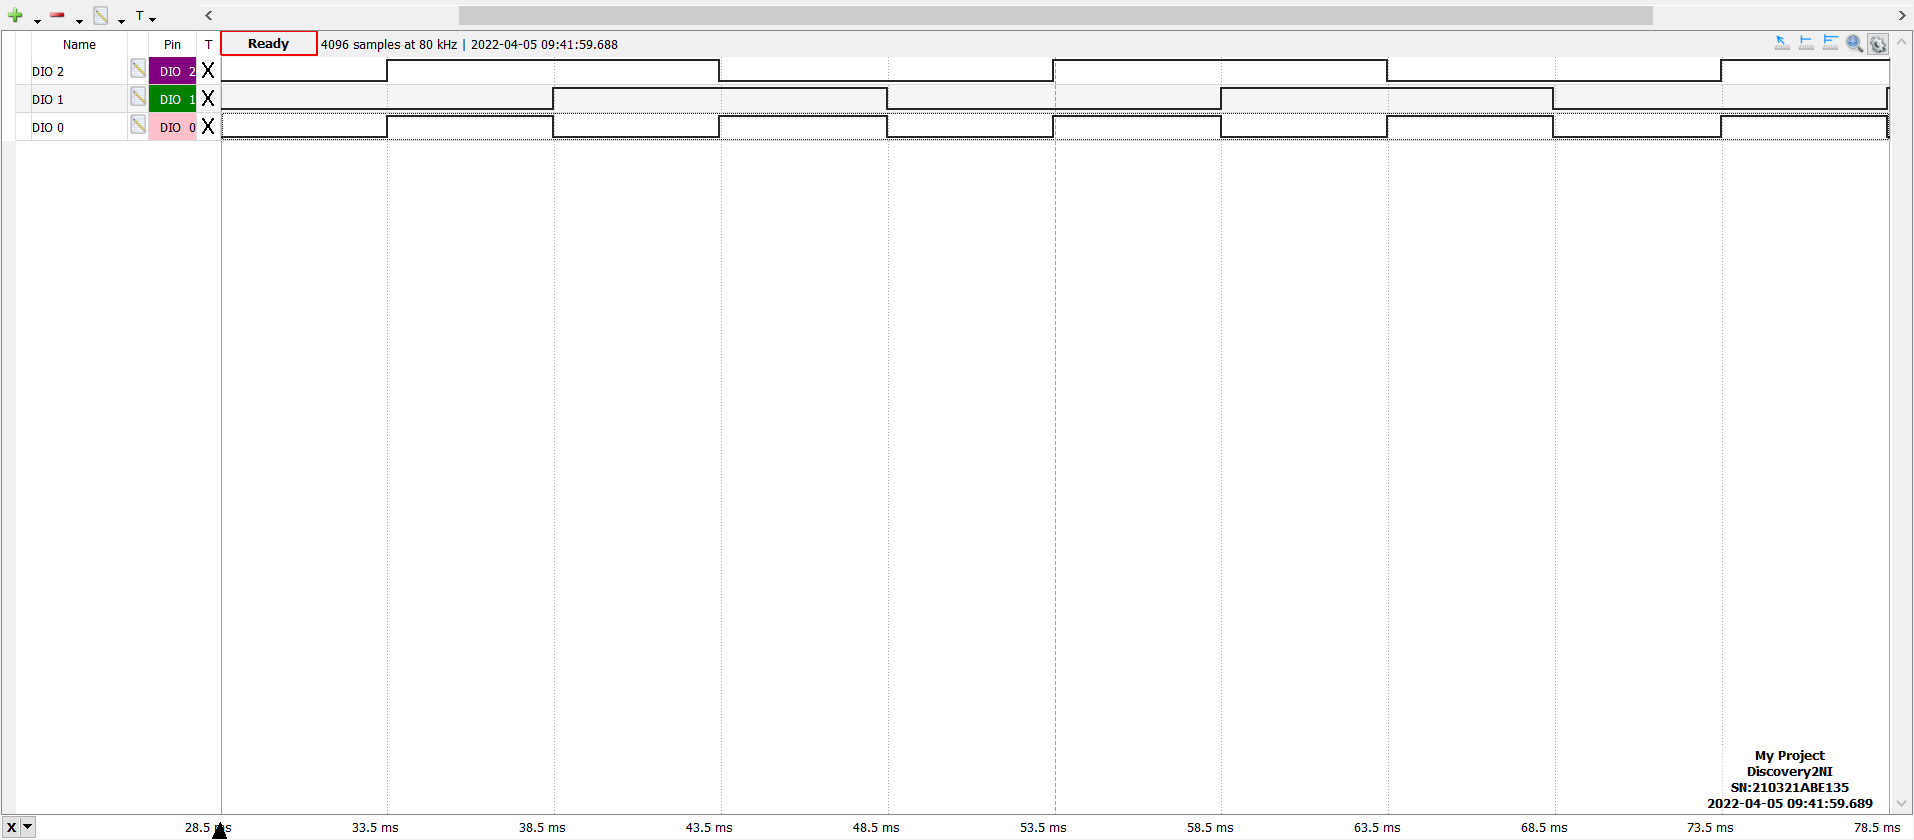
\includegraphics[width=0.8\textwidth]{xor_time}
    \caption{Acquisizione Logic della Porta XOR: DIO 0 e DIO 1 sono i segnali
    di input, DIO 2 è l'uscita dallo XOR}
    \label{fig: XOR_time}
\end{figure}
Dall'acquisizione in \ref{fig: XOR_time} osserviamo che il circuito riproduce
il comportamento atteso, in quanto l'output risulta essere L se e solo se
entrambi gli input $A$ e $B$ assumono lo stesso valore.

\setcounter{section}{5}
%=======================
\section*{Parte C: Circuiti logici complessi a più chip}
\section{Convertitore Gray-Binario}
Vogliamo costruire un circuito che converta un valore a 4 bit dalla codifica
Gray in codice Binario utilizzando un integrato di tipo SN74LS86 a porte XOR
(in \cref{fig: XOR}).
\begin{figure}[htbp]
    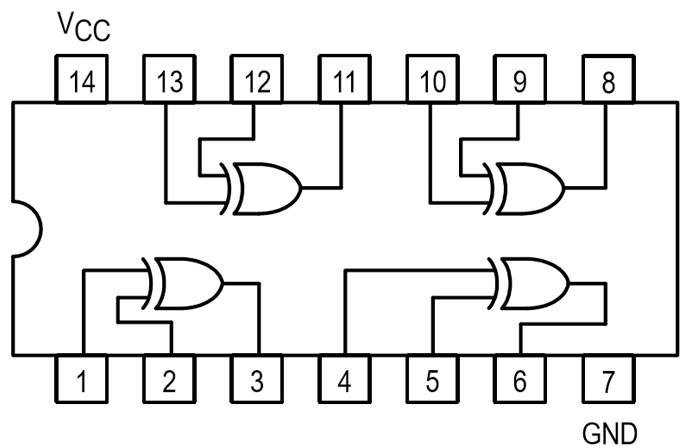
\includegraphics[width=0.3\textwidth]{XOR}
    \caption{Schema e pedinatura del circuito integrato SN74LS86 quad-XOR
    \label{fig: XOR}}
\end{figure}

Un convertitore Gray-Binario può essere schematizzato come in \cref{fig: gb},
di nuovo il nostro obiettivo è verificare che tale circuito funzioni
correttamente.
\begin{figure}[htbp]
    \centering
    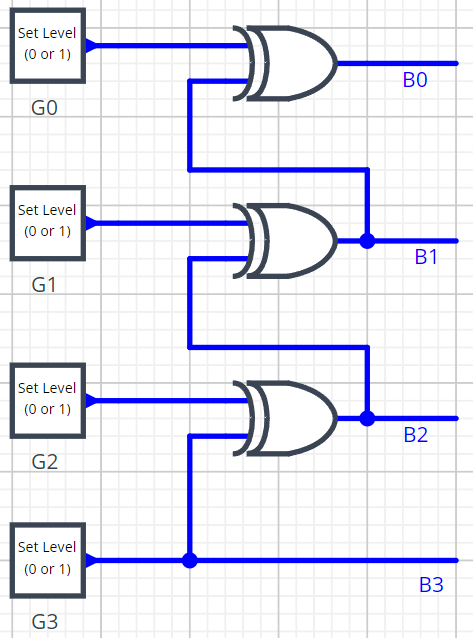
\includegraphics[width=0.5\textwidth]{gb}
    \caption{Schema logico di un circuito convertitore Gray->Binario
    \label{fig: gb}}
\end{figure}

\subsection{Verifica del disegno circuitale}
Preliminarmente possiamo calcolare i valori attesi in uscita per almeno
4 diversi stati in ingresso come verifica dello schema circuitale in
\cref{fig: gb}
\begin{table}[htbp]
    \centering
    \[
    \begin{array}{cccc|cccc}
    \toprule
        G_3 & G_2 & G_1 & G_0 & B_3 & B_2 & B_1 & B_0 \\
        \midrule
        \midrule
        0 & 0 & 0 & 0 & 0 & 0 & 0 & 0 \\
        1 & 0 & 0 & 0 & 1 & 1 & 1 & 1 \\
		1 & 0 & 0 & 1 & 1 & 1 & 1 & 0 \\        
        1 & 1 & 1 & 1 & 1 & 0 & 1 & 0 \\
    \bottomrule
    \end{array}
    \]
\end{table}

\subsection{Verifica del corretto comportamento del convertitore G->B}
Come si può vedere esplicitamente dalla \ref{tab: grbin} il codice Gray
differisce dal codice binario in quanto si passa da un numero intero al
successivo modificando un solo bit per volta.
\begin{table}[htbp]
    \centering
    \begin{tabular}{cc}
    \toprule
        Codice binario & Codice Gray \\
        \midrule
        \midrule
        0000 & 0000\\
        0001 & 0001\\
        0010 & 0011\\
        0011 & 0010\\
        0100 & 0110\\
        0101 & 0111\\
        0110 & 0101\\
        0111 & 0100\\
        1000 & 1100\\
        1001 & 1101\\
        1010 & 1111\\
        1011 & 1110\\
        1100 & 1010\\
        1101 & 1011\\
        1110 & 1001\\
        1111 & 1000\\
        \bottomrule
        \end{tabular}
    \caption{Conteggio sequenziale a 4 bit nelle due codifiche.}
    \label{tab: grbin}
\end{table}
Dunque dalla stessa possiamo vedere quali sono i valori attesi per l'uscita del
circuito al variare dei valori in ingresso.

Dunque, per conferma del corretto funzionamento del convertitore come prima
possiamo confrontare le uscite ottenute da un'acquisizione con Logic Analyzer
con i valori riportati in \cref{tab: grbin} generando all'ingresso con
Patterns un contatore Gray.
\begin{figure}[htbp]
    \centering
    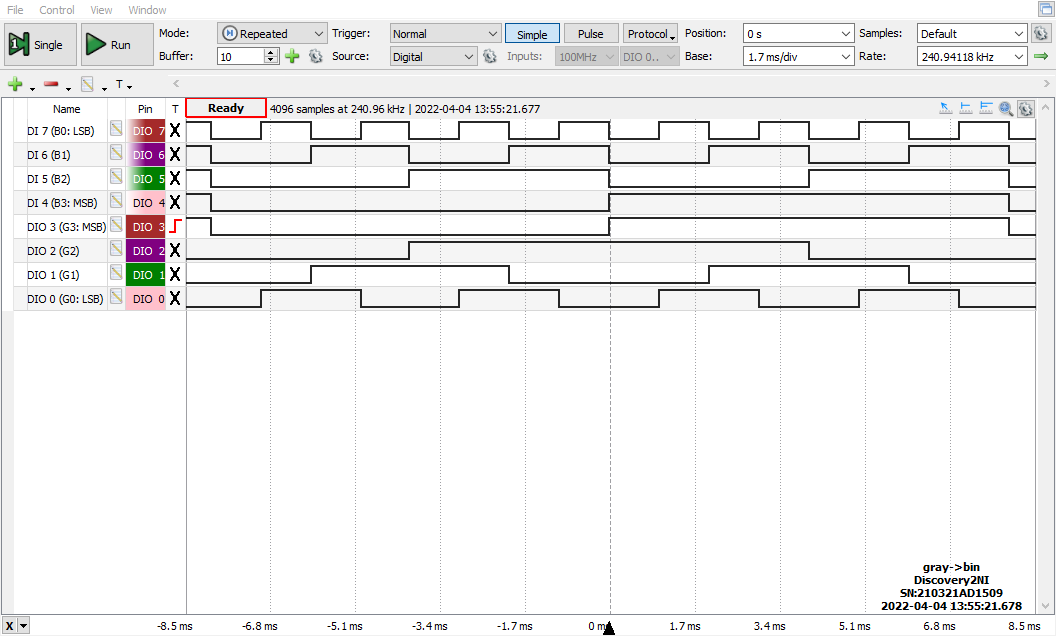
\includegraphics[width=\textwidth]{graybin}
    \caption{Acquisizione di un ciclo completo (frequenza 1 kHz) con Logic
    Analyzer dei segnali in ingresso e in uscita dal convertitore Gray-binario.}
\end{figure}

Per una scala dei tempi ristretta, abbiamo triggerato quando il MSB del bus a
codice Gray cade da H a L: in questo modo riusciamo a osservare la transizione
da 15 a 0 (1000 in Gray equivale a 1111 in binario) e in particolare il tempo
di propagazione che intercorre tra quando il segnale in ingresso scende a 0
e quando effettivamente in uscita si registra corrispondente valore in binario
(riportiamo una serie di acquisizioni di questa transizione in
\cref{fig: gray20ns} e \cref{fig: prop}
\begin{figure}[htbp]
    \centering
    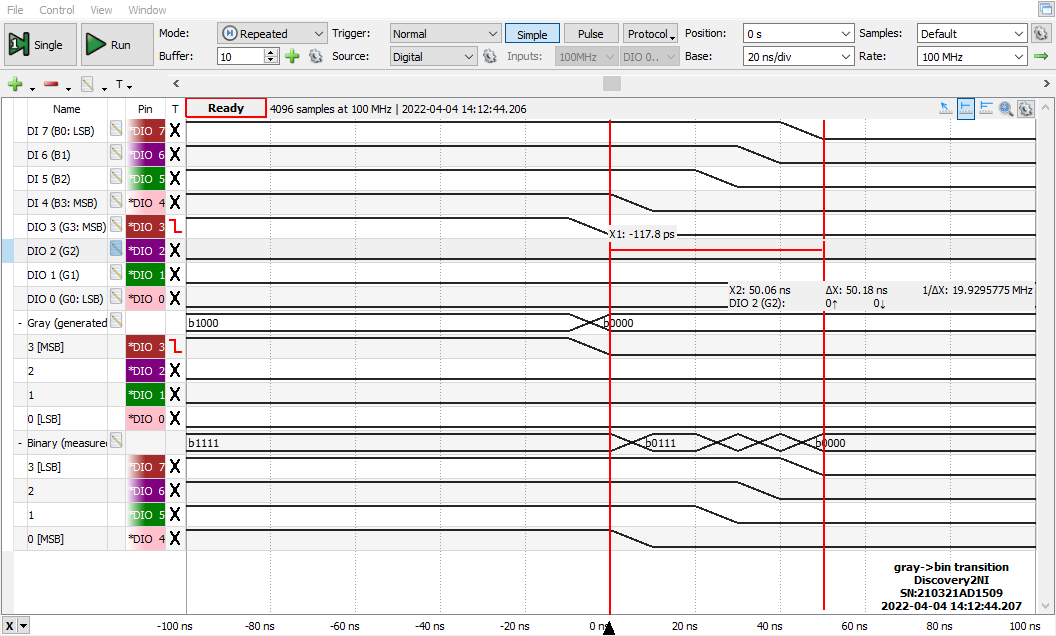
\includegraphics[width=\textwidth]{gray20ns_B}
    \caption{Acquisizione del Logic Analyzer durante la transizione dal numero
    $15$ (b1111) al numero $0$ (b0000) su scala dei tempi pari a $20$ ns.
    \label{fig: gray20ns}}
\end{figure}
\begin{figure}[htbp]
    \centering
    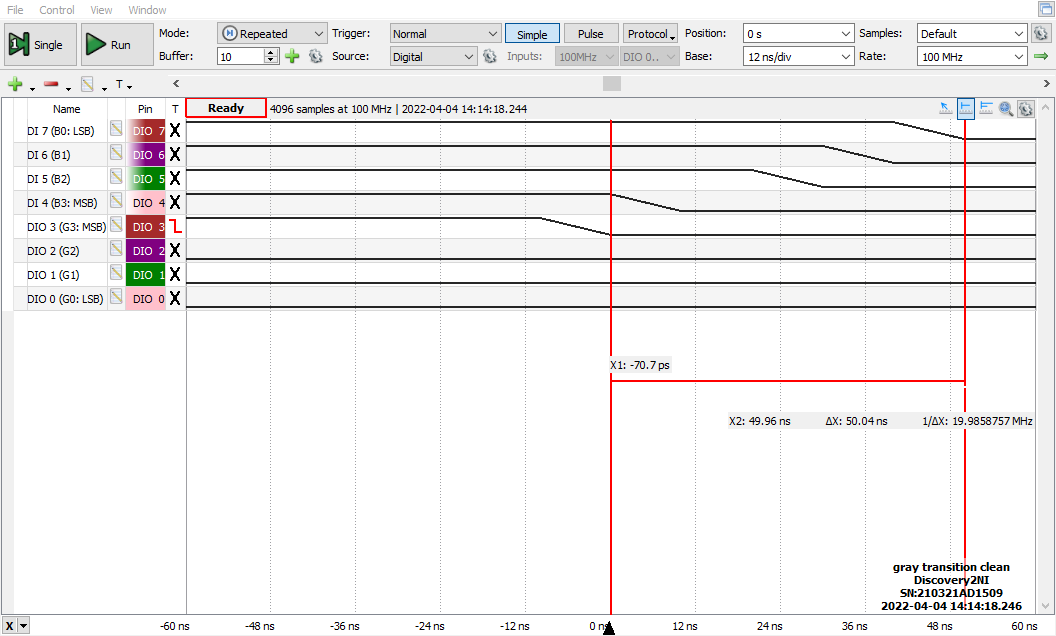
\includegraphics[width=\textwidth]{gray10ns}
    \caption{Transizione dal $15$ allo $0$ su scala temporale pari a $10$ ns.
    \label{fig: prop}}
\end{figure}

Dalla figura \cref{fig: prop} notiamo che anche se il bit 3 del segnale Gray e
il bit 3 del codice binario sono direttamente collegati tra loro
(cioè senza nessuna porta logica tra i due), quest'ultimo percepisce un
ritardo pari a circa la risoluzione temporale dell'AD2 (10 \si{n\s}).

Inoltre i successivi bit del codice binario (2, 1 e infine 0) risultano
anch'essi ognuno in ritardo rispetto al bit precedente a cui è collegato in
cascata da una porta logica XOR.

Controllando sul datasheet i tempi di propagazione per i gate XOR usati si
ricava che nel caso in cui l'altro ingresso si trovi in stato logico basso,
$t\ped{PHL, typ} = 10 \; \si{n\s}$ e $t\ped{PHL, max} = 17 \; \si{n\s}$.

Considerando quindi che il ritardo totale (da quando il bit MSB Gray scende a
0, fino a quando il bit LSB Binario scende anch'esso a 0) risulta pari a circa
$50 \pm 10 \; \si{n\s}$, questo risulta compatibile con il ritardo atteso;
ovvero quello accumulato dalle 3 porte XOR di ($\approx 30$ \si{n\s}) in
aggiunta a quello del primo bit binario (MSB) di 10 \si{n\s}.

Il ritardo "fantasma" misurato con l'AD2 presente dal momento in cui il bit
2 Binario scende a 0 fino a quando anche il bit 1 scende a 0 (indicativamente
in \cref{fig: prop} tra i 20 e i 30 \si{n\s} dopo il trigger) si ipotizza sia
da attribuire alla scarsa risoluzione dell'AD2 e ad una porta logica con tempo
di propagazione particolarmente più alto rispetto alle altre (da quanto
osservato ci aspettiamo sia lo XOR che in uscita ha il bit B1).

\section{Sommatore a 2 bit}
\subsection{Costruzione e analisi del circuito}
Vogliamo costruire un sommatore a due bit utilizzando le porte logiche
contenute nei chip integrati SN74LS08 (quad-AND), SN74LS32 (quad-OR) e
SN74LS86 (quad-XOR). Il circuito da noi costruito e studiato è riportato in
\cref{fig: sommatore}.
\begin{figure}[htbp]
    \centering
    \includegraphics[width=0.6\linewidth]{half}
    \caption{Schema logico del circuito di un half adder
    \label{fig: halfadder}}
\end{figure}

\begin{figure}[htbp]
    \centering
    \includegraphics[width=0.6\linewidth]{full}
    \caption{Schema logico del circuito di un full adder.
    \label{fig: fulladder}}
\end{figure}

\subsection{Verifica del funzionamento degli Half-Adder e Full-Adder}
Si vuole quindi verificare il funzionamento dei due circuiti Half Adder e
Full Adder schematizzati nelle \cref{fig: halfadder} e \cref{fig: fulladder}.

Per verificare il funzionamento del primo è stato sufficiente generare con
Patterns un bus contatore binario a 2 bit, inviare i segnali dei due bit a
ciascuno degli ingressi dell'HA e osservarne il comportamento con Logic
(come in \cref{fig: HA_log}).
\begin{figure}[htbp]
	\centering
	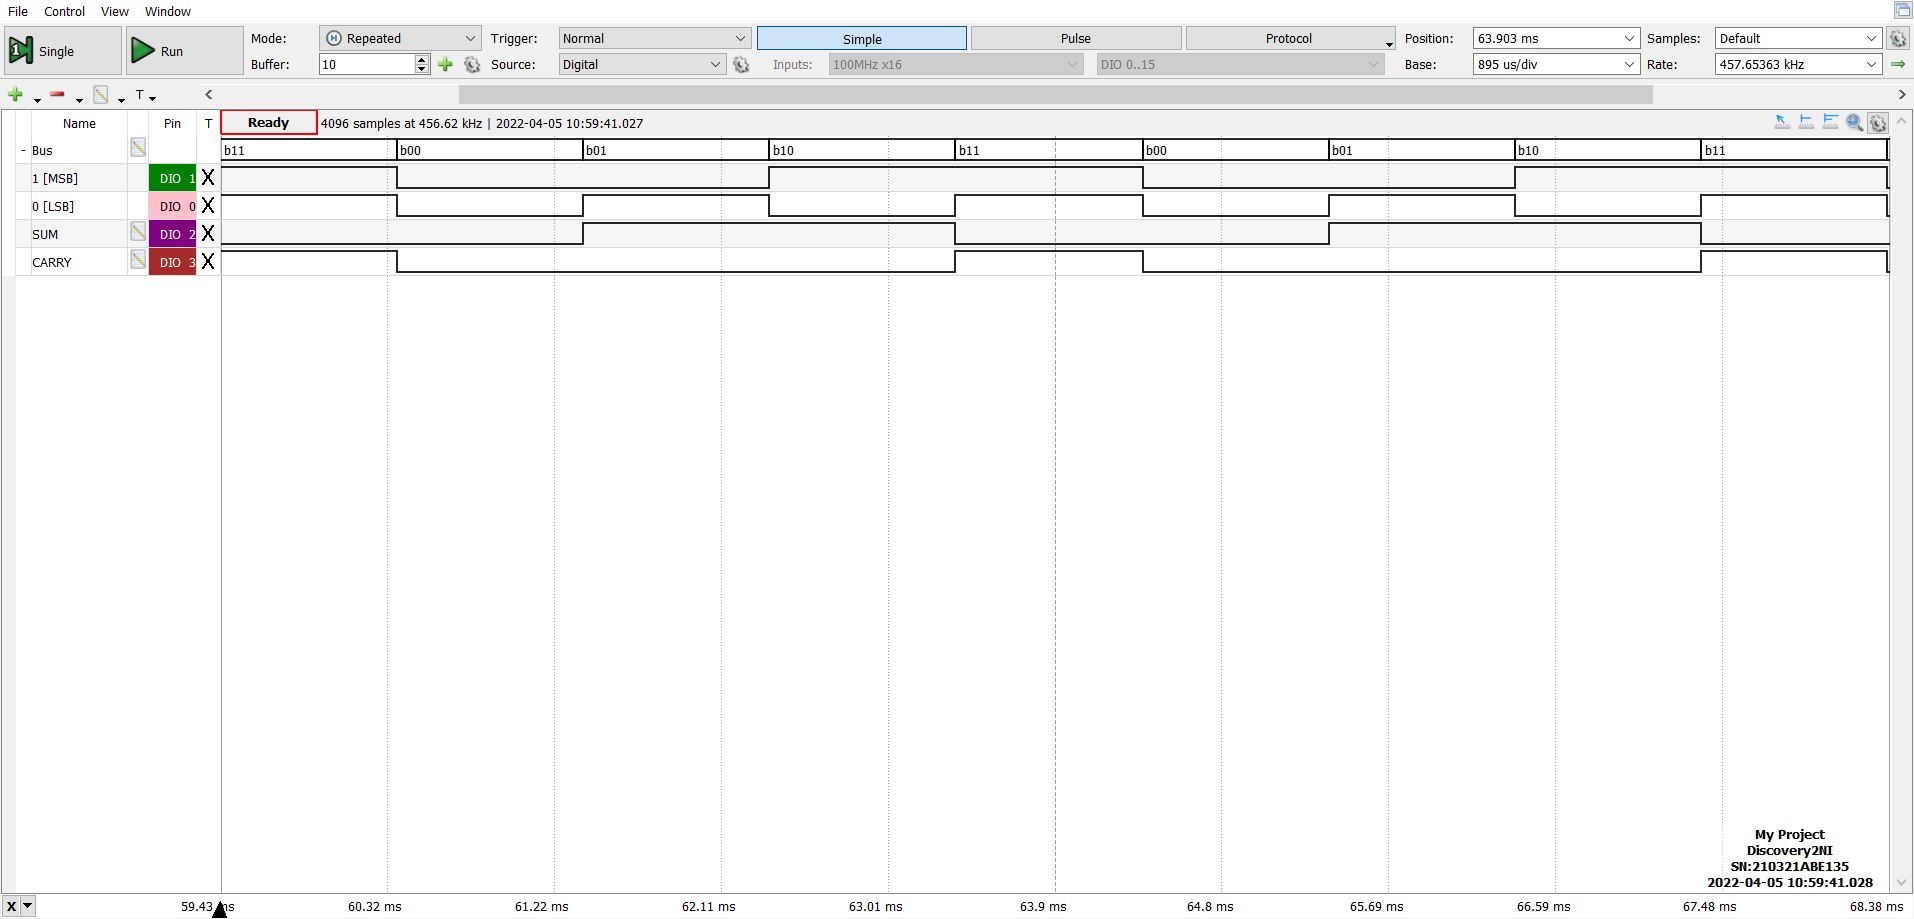
\includegraphics[width=\textwidth]{half_time}
	\caption{Acquisizione di Logic del funzionamento di un Half Adder
	\label{fig: HA_log}}
\end{figure}

Per verificare il funzionamento del Full Adder abbiamo generato con Patterns
un bus contatore (sempre in binario) a 3 bit: 2 di questi (i due bit meno
significativi) sono stati utilizzati come ingressi $A$ e $B$, mentre il MSB è
stato utilizzato come bit di CARRY IN. Riportiamo l'andamento dell'uscita del
FA in funzione dei segnali in ingresso acquisita dal Logic Analyzer in
\cref{fig: FA_log}.
\begin{figure}[htbp]
	\centering
	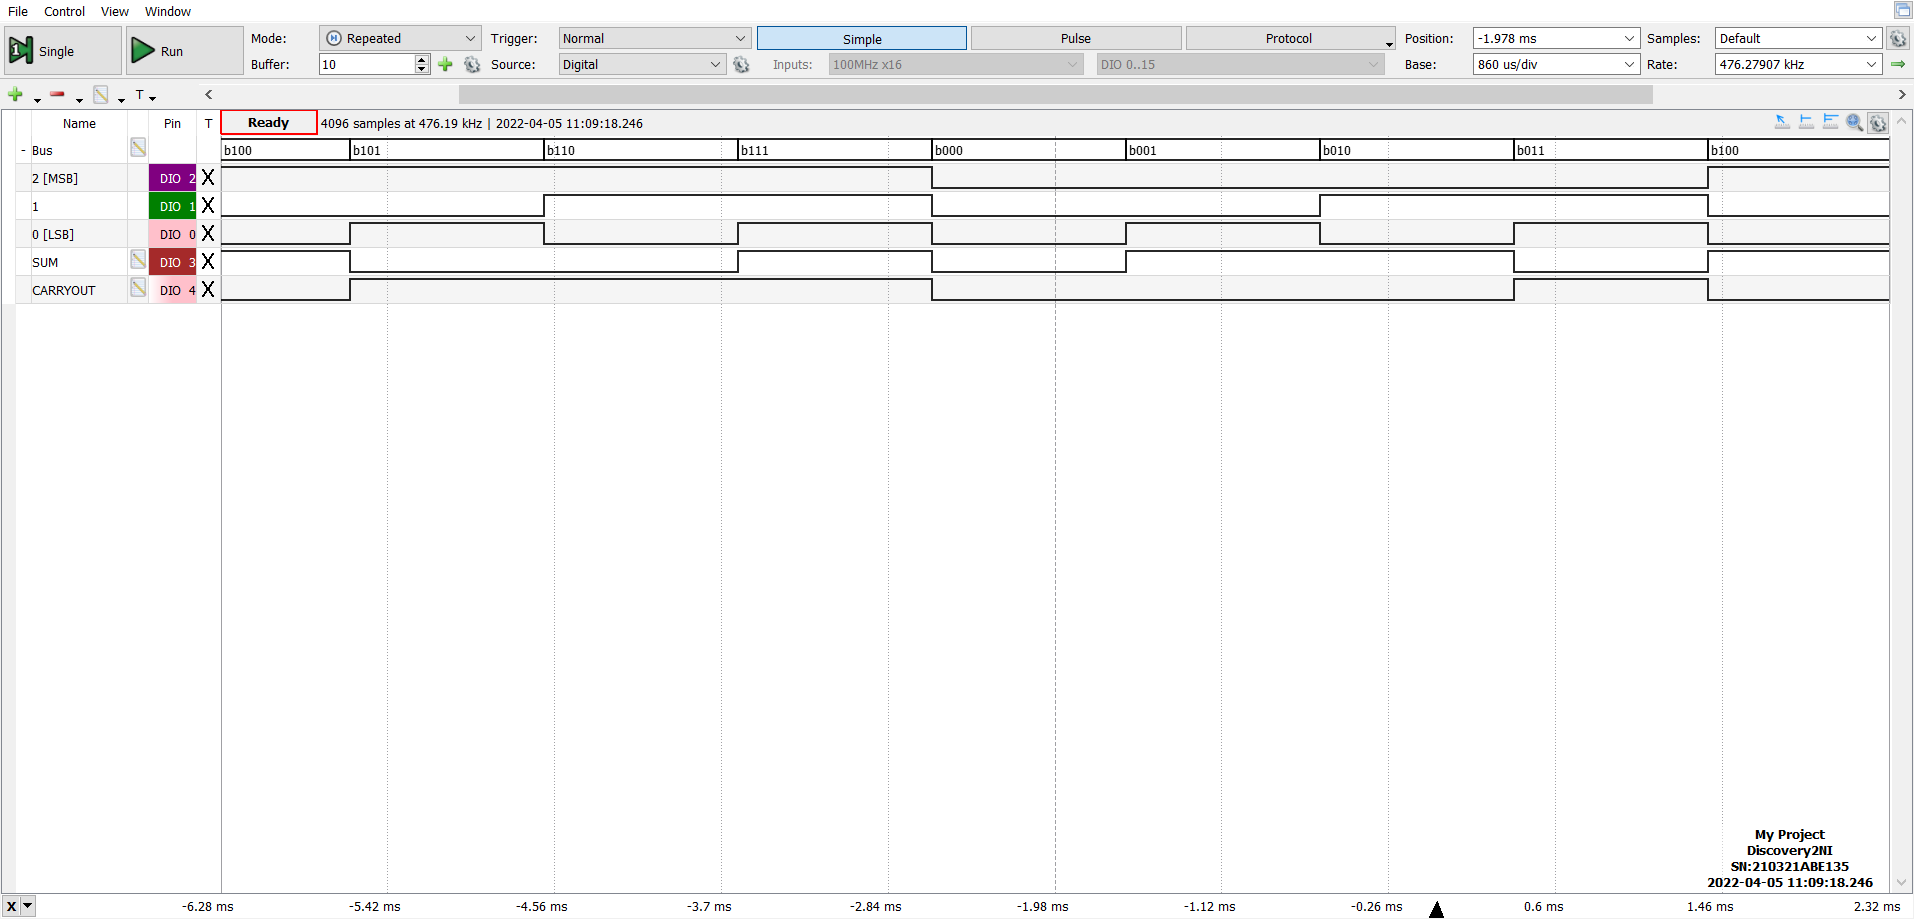
\includegraphics[width=\textwidth]{full_time}
	\caption{Acquisizione con Logic del funzionamento di un Full Adder
	\label{fig: FA_log}}
\end{figure} 
Dai risultati ottenuti con le acquisizioni di Logic si verifica che entrambi
i circuiti funzionano come ci si aspetta.

\subsection{Verifica del comportamento da sommatore con resto}
Abbiamo collegato l'uscita CARRY OUT dell'half adder all'ingresso CARRY IN
del full adder: così facendo si ottiene un sommatore binario a 2 bit con bit
di riporto (che andrà ad indicare un eventuale overflow). Riportiamo lo schema
del circuito per completezza in \cref{fig: sommatore}.
\begin{figure}[htbp]
    \centering
    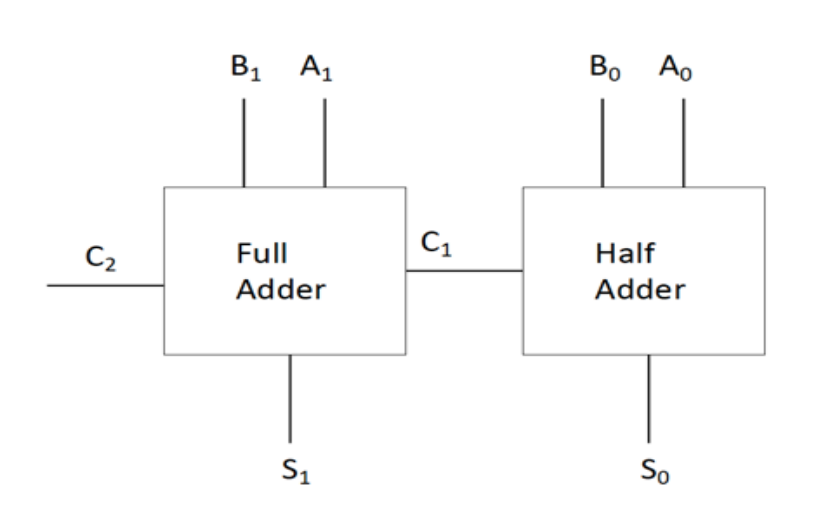
\includegraphics[width=0.6\linewidth]{sum.png}
    \caption{Schema circuitale di un sommatore a 2 bit}
    \label{fig: sommatore}
\end{figure}

A questo punto si procede con la verifica di funzionamento del circuito.
Per fare questo si genera con Patterns un Bus contatore a 4 bit che
utilizzeremo per inviare segnali corrispondenti a numeri in codice binario in
ingresso al sommatore -facendo attenzione a inserire nell'Half Adder i due
bit meno significativi di entrambi i numeri, mentre al Full Adder i due bit
più significativi- (in particolare i 2 bit meno significativi del bus
formeranno il numero $A$, mentre i restanti rappresenteranno l'intero $B$.)
\begin{figure}[htbp]
    \centering
    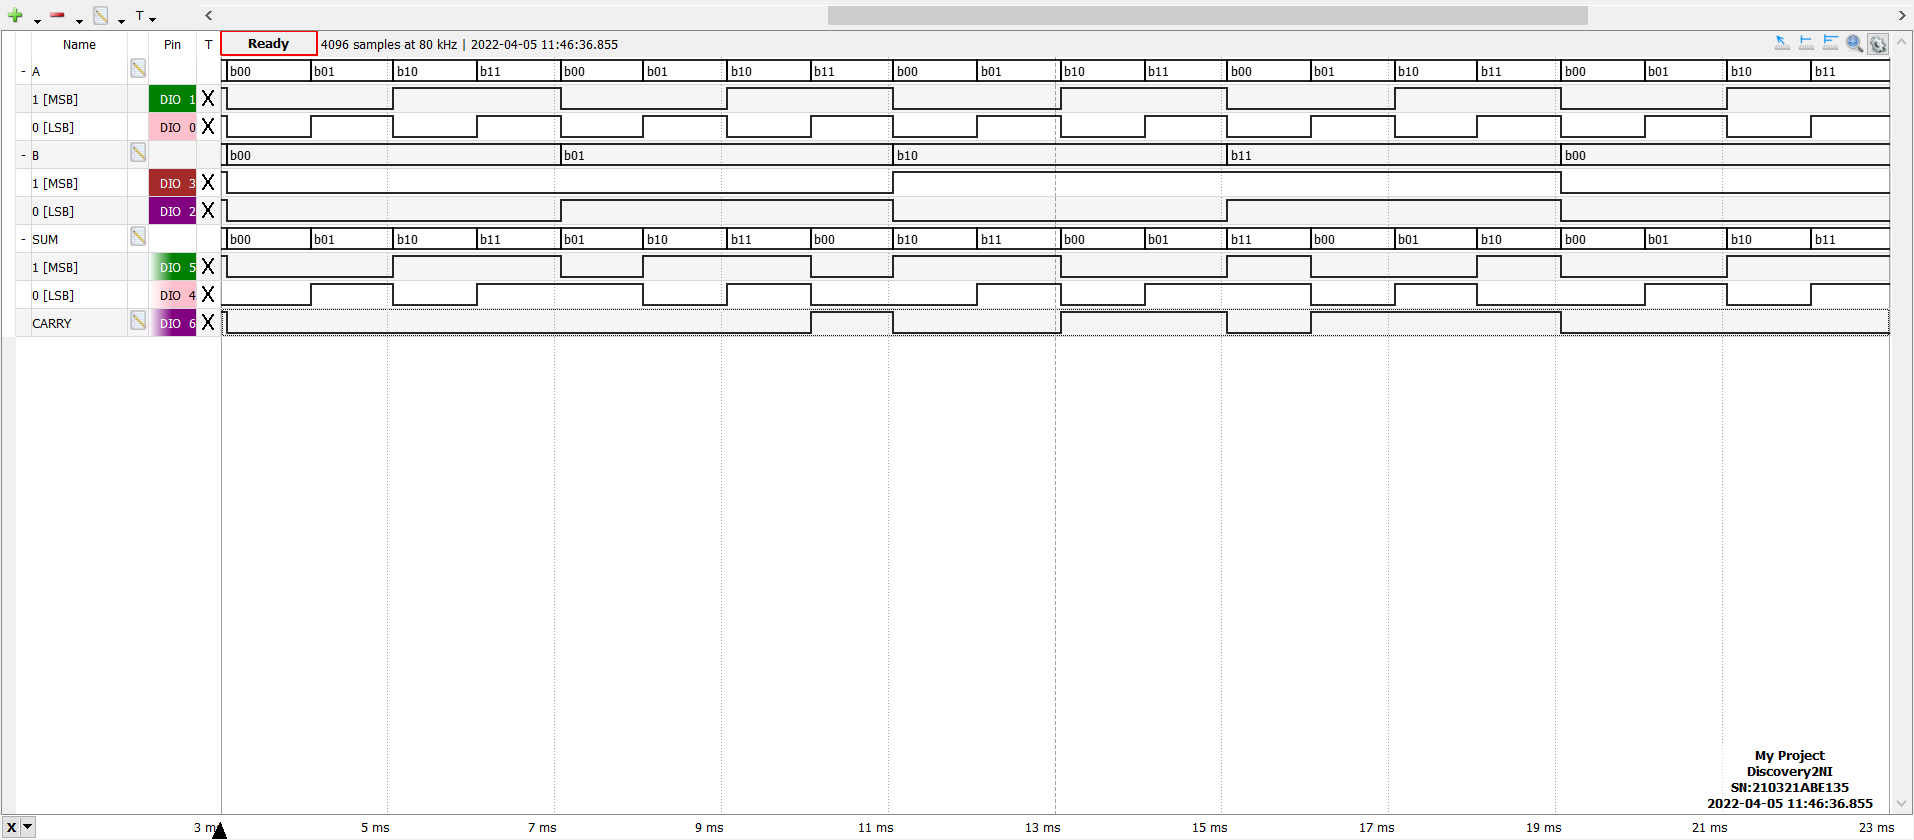
\includegraphics[width=\linewidth]{sum_time.png}
    \caption{Acquisizione con Logic per il sommatore a 2 bit: DIO 0 e DIO 1
    rappresentano il numero $A$; DIO 2 e DIO 3 rappresentano $B$; DIO 4 (LSB),
    DIO 5 (MSB) e DIO 6 (bit di overflow) rappresentano il risultato della
    somma.}
    \label{fig: faAD2}
\end{figure}
Si verifica come nei punti precedenti che il circuito sommatore si funziona
come atteso dai risultati dell'analisi con Logic riportati in
\cref{fig: faAD2}.

\subsection{Verifica funzionamento con led e ROM}
Aggiungiamo al circuito 4 led verdi e un led rosso e li colleghiamo all'AD2.
Per controllare il loro funzionamento definiamo con ROM in Patterns una
tabella di verità, riportata in \cref{fig: Ver}, tale per cui ad ogni ciclo
si illuminino un numero di led pari al valore della somma.

Il led rosso viene usato per indicare eventuale overflow, i.e. la possibilità
che il risultato sia maggiore o uguale a 4.
\begin{figure}[htbp]
    \centering
    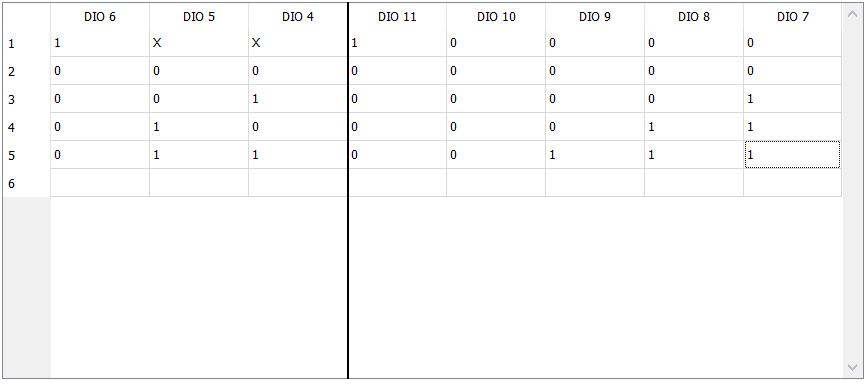
\includegraphics[width=0.8\linewidth]{TAB_LED}
    \caption{Tabella delle verità usata per il controllo dei led.
    \label{fig: Ver}}
\end{figure}

Si è fatta quindi un'ultima acquisizione tramite Logic includendo anche
i segnali inviati ai LED (riportata in \cref{fig: ROM_sommatore})
\begin{figure}[htbp]
    \centering
    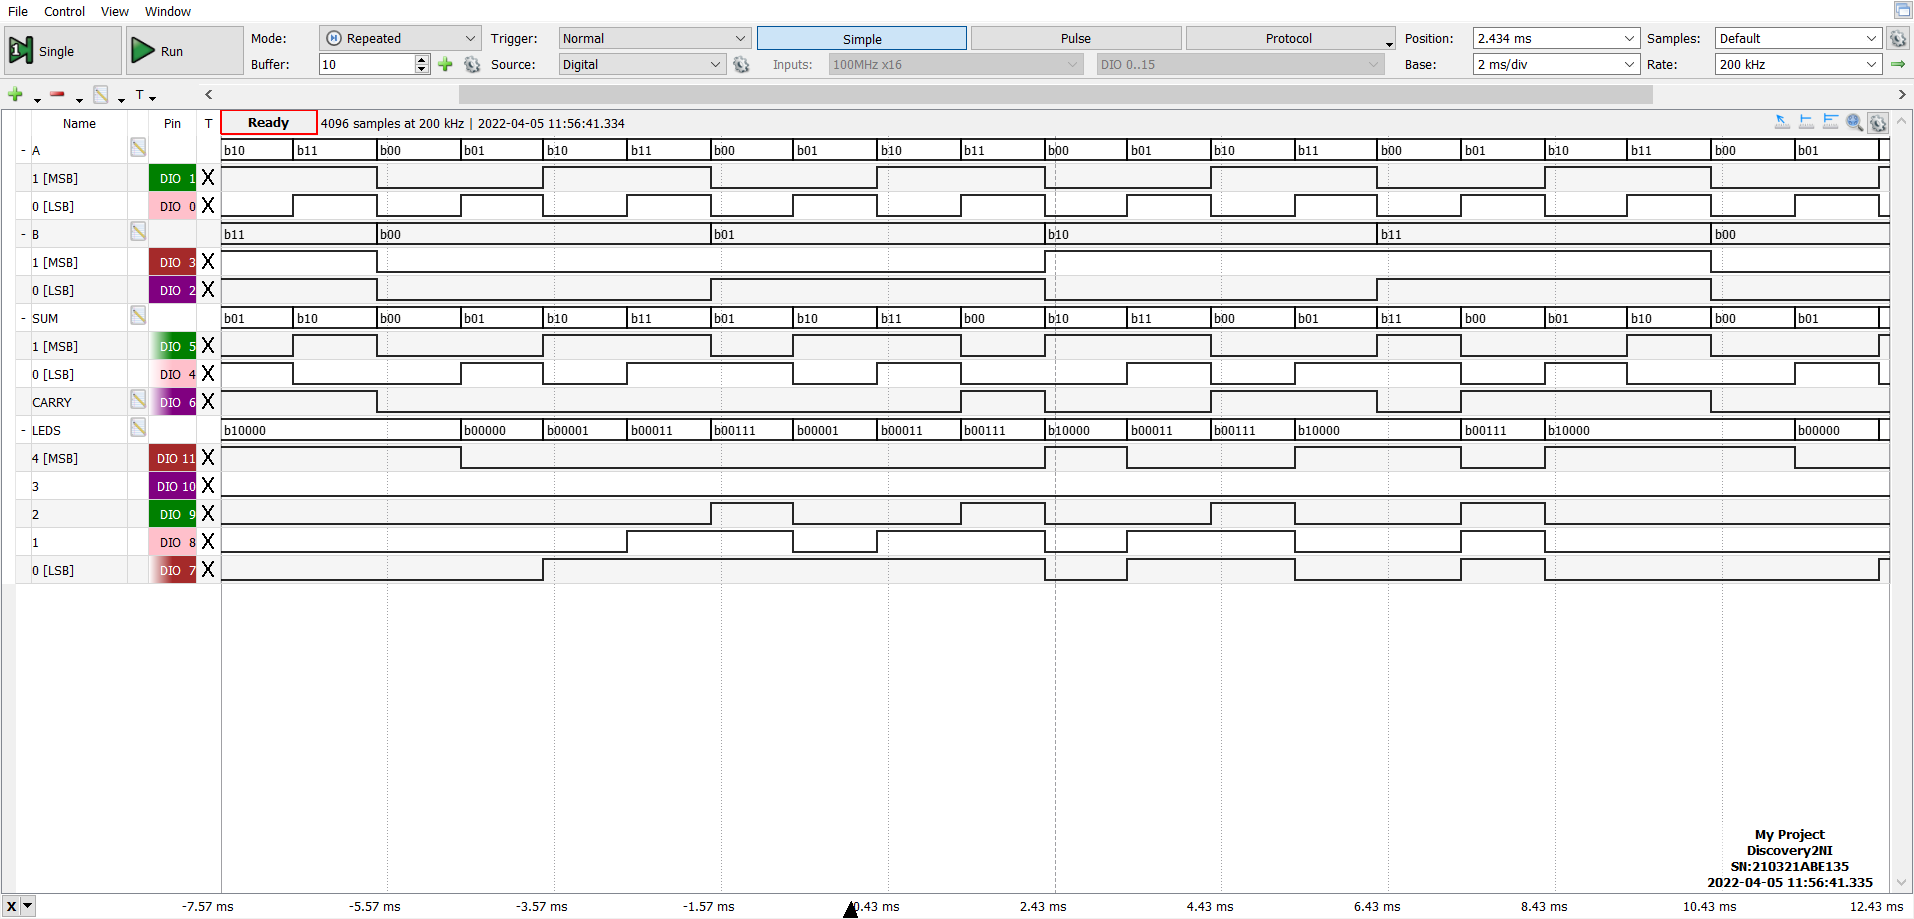
\includegraphics[width=\linewidth]{sum_time_ROM}
    \caption{Acquisizione con Logic dell'andamento nel tempo dei vari segnali
    per il circuito Sommatore a 2 bit. Il risultato in uscita dal circuito
    pilotano i led secondo la tabella di verità definita in \cref{fig: Ver}.}
    \label{fig: ROM_sommatore}
\end{figure}
Compatibilmente con quanto ci si aspettava l'ultimo LED verde non si accende
mai (dato che con 2 bit è possibile a rappresentare solo i numeri fino a 3) e
osserviamo solo il LED rosso accendersi quando il bit di CARRY ha valore logico
alto.

%=======================
\section*{Conclusioni e commenti finali}
Si è riusciti a verificare il corretto comportamento delle porte TTL studiate
caratterizzandone le tensioni, correnti di operazione e tempi caratteristici
di circuiti integrati come il SN7404.
Inoltre, è stato possibile verificare il funzionamento di circuiti logici di
diversa complessità costruiti con porte NAND, XOR, e OR e si è riusciti ad
apprezzare l'effetto dei tempi di propagazione delle porte nella conversione
dalla codifica Gray al binario.

%=======================
\section*{Dichiarazione}
I firmatari di questa relazione dichiarano che il contenuto della relazione \`e
originale, con misure effettuate dai membri del gruppo, e che tutti i firmatari
hanno contribuito alla elaborazione della relazione stessa.

\end{document}
